\def\DTExplainerLanguage{en}
\documentclass[11pt,a4paper]{article}
% Shared visual and semantic style for the D-Tracker explainers.
\NeedsTeXFormat{LaTeX2e}
\RequirePackage{etoolbox}
\providecommand{\DTExplainerLanguage}{en}

\ifdefstring{\DTExplainerLanguage}{vi}{%
  \RequirePackage[main=vietnamese,english]{babel}%
}{%
  \RequirePackage[main=english]{babel}%
}

\RequirePackage{fontspec}
\setmainfont{TeXGyrePagellaX-Regular.otf}[
  BoldFont=TeXGyrePagellaX-Bold.otf,
  ItalicFont=TeXGyrePagellaX-Italic.otf,
  BoldItalicFont=TeXGyrePagellaX-BoldItalic.otf
]
\setsansfont{texgyreheros-regular.otf}[
  BoldFont=texgyreheros-bold.otf,
  ItalicFont=texgyreheros-italic.otf,
  BoldItalicFont=texgyreheros-bolditalic.otf
]
\setmonofont{texgyrecursor-regular.otf}[
  BoldFont=texgyrecursor-bold.otf,
  ItalicFont=texgyrecursor-italic.otf,
  BoldItalicFont=texgyrecursor-bolditalic.otf,
  Scale=0.85
]
\RequirePackage{unicode-math}
\setmathfont{texgyrepagella-math.otf}
\setmathfont[version=bold,FakeBold=1.15]{texgyrepagella-math.otf}

\RequirePackage[a4paper,top=24mm,bottom=24mm,left=23mm,right=23mm,headheight=22pt]{geometry}
\RequirePackage{microtype}
\RequirePackage{amsmath,bm}
\RequirePackage{graphicx}
\RequirePackage{xcolor}
\RequirePackage[breakable,skins]{tcolorbox}
\RequirePackage{booktabs,longtable,array,tabularx,multirow}
\RequirePackage{enumitem}
\RequirePackage{caption}
\RequirePackage{subcaption}
\RequirePackage{titlesec}
\RequirePackage{fancyhdr}
\RequirePackage{tikz}
\usetikzlibrary{arrows.meta,positioning,fit,shapes.geometric,calc,backgrounds,decorations.pathreplacing}
\definecolor{DTNavy}{HTML}{16324F}
\definecolor{DTTeal}{HTML}{0F7C7B}
\definecolor{DTGold}{HTML}{C58B1B}
\definecolor{DTClaret}{HTML}{8C2F39}
\definecolor{DTInk}{HTML}{23313D}
\definecolor{DTMist}{HTML}{EEF4F4}
\definecolor{DTWarm}{HTML}{FBF4E4}
\definecolor{DTPaper}{HTML}{FCFCFA}
\RequirePackage[colorlinks=true,linkcolor=DTTeal,citecolor=DTTeal,urlcolor=DTNavy]{hyperref}
\RequirePackage{bookmark}
\RequirePackage[nameinlink,noabbrev]{cleveref}

\color{DTInk}
\pagecolor{DTPaper}
\setlength{\parindent}{0pt}
\setlength{\parskip}{0.55em plus 0.15em minus 0.1em}
\linespread{1.06}
\setlist[itemize]{leftmargin=1.35em,itemsep=0.25em,topsep=0.35em}
\setlist[enumerate]{leftmargin=1.55em,itemsep=0.3em,topsep=0.35em}
\captionsetup{font=small,labelfont={bf,color=DTNavy},justification=raggedright,singlelinecheck=false}
\setlength{\emergencystretch}{2.5em}

\titleformat{\section}
  {\sffamily\LARGE\bfseries\color{DTNavy}}{\thesection}{0.65em}{}
  [\vspace{2pt}{\color{DTTeal}\titlerule[1.1pt]}]
\titleformat{\subsection}
  {\sffamily\Large\bfseries\color{DTTeal}}{\thesubsection}{0.55em}{}
\titleformat{\subsubsection}
  {\sffamily\large\bfseries\color{DTNavy}}{\thesubsubsection}{0.5em}{}
\titlespacing*{\section}{0pt}{2.3ex plus 0.4ex}{1.2ex}
\titlespacing*{\subsection}{0pt}{1.8ex plus 0.3ex}{0.8ex}
\titlespacing*{\subsubsection}{0pt}{1.3ex plus 0.2ex}{0.6ex}

\pagestyle{fancy}
\fancyhf{}
\fancyhead[L]{\sffamily\footnotesize\color{DTNavy}\DTShortTitle}
\fancyhead[R]{\sffamily\footnotesize\color{DTNavy}\DTLanguageName}
\fancyfoot[C]{\sffamily\footnotesize\color{DTNavy}\thepage}
\renewcommand{\headrulewidth}{0.35pt}
\renewcommand{\headrule}{\hbox to\headwidth{\color{DTTeal}\leaders\hrule height \headrulewidth\hfill}}
\fancypagestyle{plain}{%
  \fancyhf{}%
  \fancyfoot[C]{\sffamily\footnotesize\color{DTNavy}\thepage}%
  \renewcommand{\headrulewidth}{0pt}%
}

\newtcolorbox{keypoint}{
  enhanced, breakable, colback=DTMist, colframe=DTTeal,
  boxrule=0.65pt, arc=2mm, left=3mm, right=3mm, top=2mm, bottom=2mm,
  title={\sffamily\bfseries\DTKeyPointName}, fonttitle=\small,
  coltitle=white, colbacktitle=DTTeal, attach boxed title to top left={xshift=4mm,yshift=-2mm},
  boxed title style={arc=1mm,boxrule=0pt},
  before skip=1.0em, after skip=1.0em
}
\newtcolorbox{plainwords}{
  enhanced, breakable, colback=white, colframe=DTGold,
  boxrule=0.65pt, arc=2mm, left=3mm, right=3mm, top=2mm, bottom=2mm,
  title={\sffamily\bfseries\DTPlainWordsName}, fonttitle=\small,
  coltitle=white, colbacktitle=DTGold, attach boxed title to top left={xshift=4mm,yshift=-2mm},
  boxed title style={arc=1mm,boxrule=0pt},
  before skip=1.0em, after skip=1.0em
}
\newtcolorbox{commonmistake}{
  enhanced, breakable, colback=DTWarm, colframe=DTClaret,
  boxrule=0.65pt, arc=2mm, left=3mm, right=3mm, top=2mm, bottom=2mm,
  title={\sffamily\bfseries\DTMistakeName}, fonttitle=\small,
  coltitle=white, colbacktitle=DTClaret, attach boxed title to top left={xshift=4mm,yshift=-2mm},
  boxed title style={arc=1mm,boxrule=0pt},
  before skip=1.0em, after skip=1.0em
}
\newtcolorbox{selfcheck}{
  enhanced, breakable, colback=white, colframe=DTNavy,
  boxrule=0.75pt, arc=2mm, left=3mm, right=3mm, top=2mm, bottom=2mm,
  title={\sffamily\bfseries\DTSelfCheckName}, fonttitle=\small,
  coltitle=white, colbacktitle=DTNavy, attach boxed title to top left={xshift=4mm,yshift=-2mm},
  boxed title style={arc=1mm,boxrule=0pt},
  before skip=1.0em, after skip=1.0em
}

\newcommand{\sourcefig}[4][width=\linewidth]{%
  \begin{figure}[htbp]
    \centering
    \includegraphics[#1]{figures/#2}%
    \caption{#3\\[3pt]\footnotesize\textit{\DTFigureSource}}%
    \label{#4}%
  \end{figure}%
}

\newcommand{\term}[2]{\textbf{#1} (#2)}
\newcommand{\paper}[1]{\textsf{\small[#1]}}
\newcommand{\bigidea}[1]{%
  \begin{keypoint}#1\end{keypoint}%
}
\newcommand{\DTTitlePage}{%
  \begin{titlepage}
    \thispagestyle{empty}
    \vspace*{0.06\textheight}
    {\color{DTTeal}\rule{\textwidth}{2.4pt}}\\[5mm]
    {\sffamily\bfseries\color{DTNavy}\fontsize{33}{38}\selectfont \DTTitle\par}
    \vspace{5mm}
    {\sffamily\Large\color{DTTeal}\DTSubtitle\par}
    \vfill
    \begin{tcolorbox}[enhanced,colback=DTMist,colframe=DTMist,arc=2mm,boxrule=0pt,left=5mm,right=5mm,top=4mm,bottom=4mm]
      {\sffamily\bfseries\color{DTNavy}\DTPaperTitle\par}
      \vspace{2mm}
      {\small Shingo Higashiguchi, Yasuko Matsubara, Koki Kawabata,\\
      Taichi Murayama, Yasushi Sakurai\par}
      \vspace{2mm}
      {\footnotesize KDD '25 \textperiodcentered\ arXiv:2505.00242v1 \textperiodcentered\ DOI 10.1145/3690624.3709192\par}
    \end{tcolorbox}
    \vspace{8mm}
    {\small\raggedright\color{DTClaret}\DTDisclaimer\par}
    \vfill
    {\sffamily\small\color{DTNavy}\DTAuthorLine\par}
    \vspace{4mm}
    {\sffamily\small\color{DTNavy}\DTDate\par}
    \vspace*{0.04\textheight}
    {\color{DTTeal}\rule{\textwidth}{0.8pt}}
  \end{titlepage}%
}

\AtBeginDocument{%
  \hypersetup{
    pdftitle={\DTTitle},
    pdfauthor={D-Tracker explainer},
    pdfsubject={Explanation of D-Tracker for first-time readers},
    pdfkeywords={D-Tracker, tensor stream, reaction-diffusion, forecasting}
  }%
}


\newcommand{\DTLanguageName}{English}
\newcommand{\DTShortTitle}{D-Tracker --- a first-principles guide}
\newcommand{\DTTitle}{D-Tracker}
\newcommand{\DTSubtitle}{Understanding the paper from its first ideas}
\newcommand{\DTPaperTitle}{Modeling Interest Diffusion in Social Activity Tensor Data Streams}
\newcommand{\DTDisclaimer}{This is an independent explanatory document, not a translation or a substitute for the paper. Read it alongside arXiv:2505.00242v1.}
\newcommand{\DTAuthorLine}{A study guide for the CS313 project}
\newcommand{\DTDate}{25 November 2026}
\newcommand{\DTKeyPointName}{Key idea}
\newcommand{\DTPlainWordsName}{In plain words}
\newcommand{\DTMistakeName}{Common mistake}
\newcommand{\DTSelfCheckName}{Check yourself}
\newcommand{\DTFigureSource}{Image source: Higashiguchi et al. (2025), arXiv:2505.00242v1; author-owned figure, CC BY 4.0.}
\newcommand{\DTReferencesName}{Source and further reading}

\begin{document}
\hypersetup{pageanchor=false}
\DTTitlePage
\hypersetup{pageanchor=true}

\pagenumbering{roman}
\section*{How to read this document}
This guide is written for a reader who has never studied a tensor-stream paper. You do not
need to know reaction--diffusion equations, tensor factorization, or MDL beforehand: each
idea begins with a small example, then moves to the formula and its role in the paper. The
boxes \textbf{Key idea}, \textbf{In plain words}, \textbf{Common mistake}, and
\textbf{Check yourself} can be read independently for quick revision. Notation follows the
paper; a symbol table is provided in the appendix.

\tableofcontents
\clearpage

\pagenumbering{arabic}
\section{Orientation: what problem does the paper solve?}
\label{sec:orientation}

Imagine that you manage a campaign for a new phone. You have weekly search volumes for a few
keywords in many countries. Three natural questions arise:

\begin{enumerate}
  \item \textbf{Where?} Which countries are most interested in each product?
  \item \textbf{From where to where?} If interest rises in the United States and rises a few
        weeks later in Vietnam, is that a sign of diffusion?
  \item \textbf{What next?} What will interest look like next week or next month in each place?
\end{enumerate}

D-Tracker is designed to answer these questions together on a \emph{tensor stream}, not merely
on a simple time-series table. Its central idea is not a large neural forecast. It is a small,
physically meaningful model that compresses the data while exposing the changing patterns.

\begin{keypoint}
D-Tracker decomposes observations into \textbf{trend + seasonal + outlier}. The trend is compressed
into a small core, and that core evolves under a \textbf{reaction--diffusion} system that represents
growth and spread across location groups. The model is updated as data arrive and switches to a
new model when the structure changes.
\end{keypoint}

\subsection{A small example with three kinds of signal}

Table~\ref{tab:running-example} is \textbf{an illustrative example created for this guide}, not a
result from the paper. Each cell is an interest index from 0 to 100.

\begin{table}[htbp]
  \centering
  \small
  \caption{Illustrative example: one keyword has different interest across locations and time.}
  \label{tab:running-example}
  \begin{tabular}{llrrr}
    \toprule
    Keyword & Location & Week 1 & Week 2 & Week 3 \\
    \midrule
    iPhone & United States & 80 & 84 & 90 \\
    iPhone & Vietnam & 15 & 22 & 35 \\
    Galaxy & United States & 45 & 40 & 32 \\
    Galaxy & Vietnam & 30 & 34 & 40 \\
    \bottomrule
  \end{tabular}
\end{table}

At least three things are happening. First, ``iPhone'' rises in both places, but more strongly in
the United States. Second, the rise in Vietnam follows the United States in this example --- a
\emph{candidate} for interest diffusion, not evidence of causation. Third, ``Galaxy'' falls in the
United States while rising in Vietnam, so the trend is not the same for every keyword--location
pair. Real data also contain seasonality (product launches, year-end sales) and sudden spikes.

\begin{plainwords}
Looking at one line makes it easy to confuse seasonality with trend and a one-off spike with
diffusion. D-Tracker first separates the three sources of signal, then looks for structure in the
trend part.
\end{plainwords}

\subsection{Three challenges and three promises}

The paper emphasizes three difficulties. The data have \textbf{complex patterns} (trend,
seasonality, diffusion, outliers); those patterns \textbf{change over time}; and the data form a
high-dimensional tensor that is \textbf{semi-infinite} in time. The authors summarize their answer
with three properties in the introduction and conclusion:

\begin{description}[leftmargin=1.8em,style=nextline]
  \item[Interpretable.] The latent core and non-negative factors show which location/keyword groups
  relate to each dynamics and in which direction interest spreads. This is interpretability
  \emph{through model structure}, not a proof of causal effects.
  \item[Automatic.] The latent dimensions and model-switch times are selected with a compression
  criterion (MDL), rather than asking a user to try configurations by hand. Numerical optimizers
  still have settings; the user does not manually choose ``two groups or three?'' for each period.
  \item[Scalable.] Each update processes only a fixed-length recent window, so runtime does not grow
  with the total length of the stream. The paper reports being up to 8.0$\times$ faster and ``up to
  57\% improvement'' than competitors. The 57\% sentence names neither the metric nor its
  denominator, so these are paper claims, not a normalized effect size or a reproduction in this repo.
\end{description}

\begin{commonmistake}
``Scalable'' here does not mean that every operation is $O(1)$. It means that processing one stream
step does not depend on how long the stream has already become, because only a window is retained.
Cost still grows with the number of keywords, locations, and latent dimensions.
\end{commonmistake}

\subsection{See the result before learning the machinery}

\begin{figure}[htbp]
  \centering
  \begin{subfigure}[t]{0.92\linewidth}
    \centering
    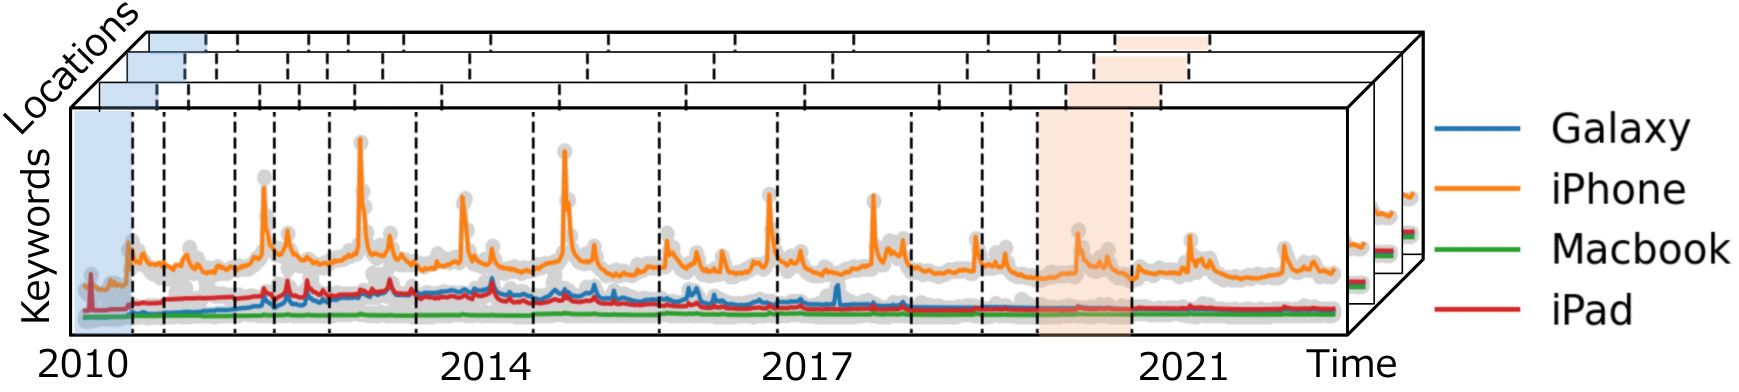
\includegraphics[width=\linewidth]{figures/Figure1_a.png}
    \caption{Observations (gray) and model fit (color); dotted vertical lines mark model switches.}
  \end{subfigure}

  \vspace{4mm}
  \begin{subfigure}[t]{0.82\linewidth}
    \centering
    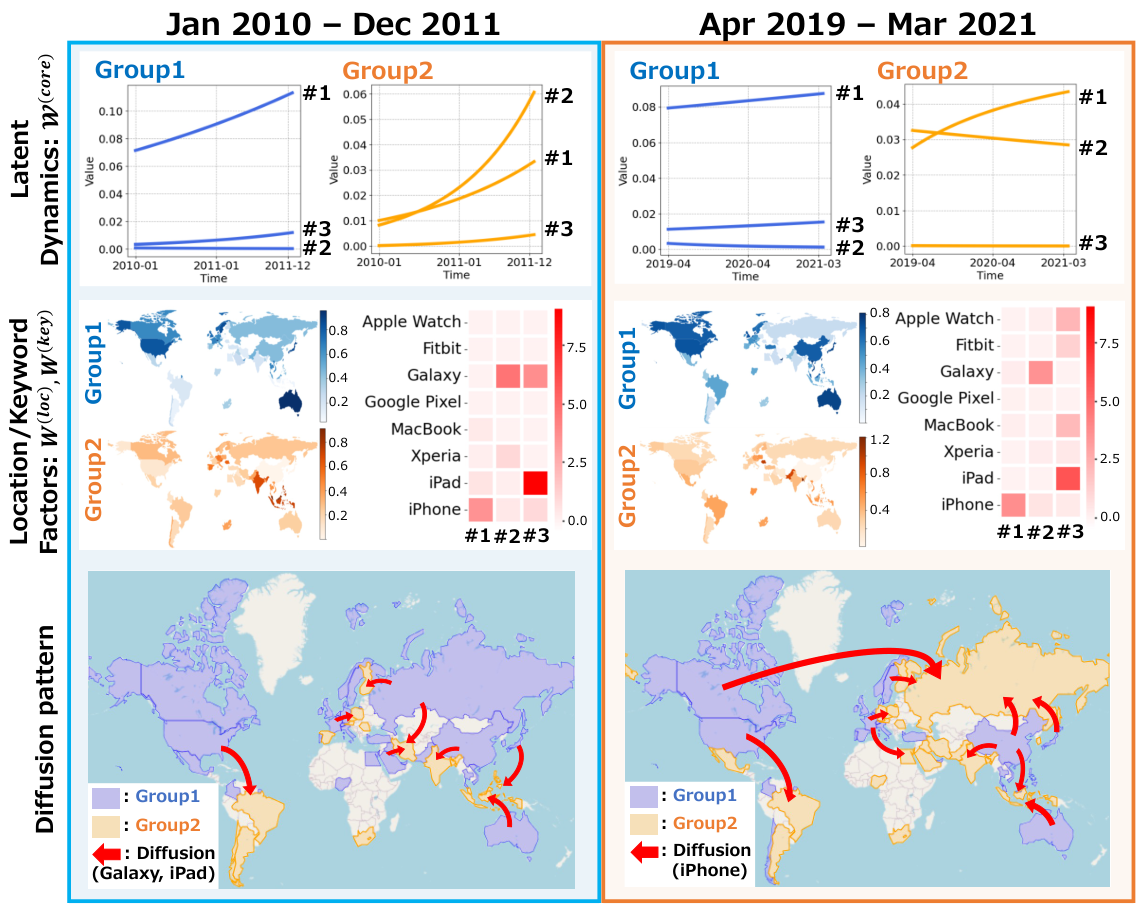
\includegraphics[width=\linewidth]{figures/Figure1_b.png}
    \caption{Latent dynamics, location/keyword factors, and diffusion maps in two periods.}
  \end{subfigure}
  \caption{Modeling power of D-Tracker on the device data. Source: Higashiguchi et al. (2025),
  arXiv:2505.00242v1, Figure~1; author-owned figure, CC BY 4.0.}
  \label{fig:preview}
\end{figure}

In Figure~\ref{fig:preview}(a), the model does not use one parameter set for the whole displayed period. The
dotted lines split the stream into periods, each modeled separately. This is \emph{regime switching}.
In Figure~\ref{fig:preview}(b), each column is one dynamics: the top curve is the core
$\mathcal{W}^{(\mathrm{core})}$ over time; the middle row shows how strongly that dynamics relates
to keywords and location groups; the bottom row shows diffusion arrows between groups. We therefore
get more than a forecast: a testable story about which dynamics, keyword, region, and direction.

\begin{figure}[htbp]
  \centering
  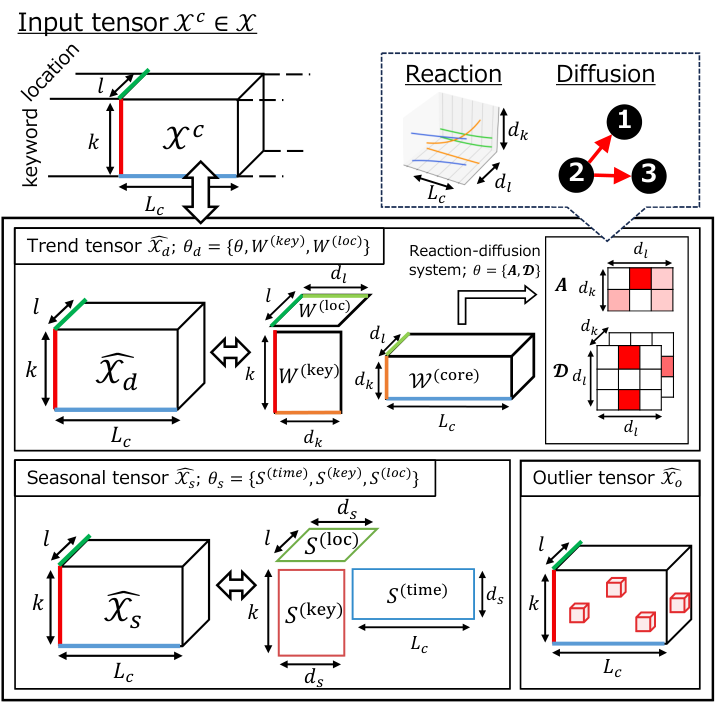
\includegraphics[width=0.72\linewidth]{figures/overview.png}
  \caption{D-Tracker overview: the current tensor is approximated by trend + seasonal + outlier.
  Source: Higashiguchi et al. (2025), arXiv:2505.00242v1, Figure~2; author-owned figure, CC BY 4.0.}
  \label{fig:overview}
\end{figure}

Figure~\ref{fig:overview} is the map of the whole paper. The input is the current tensor
$\mathcal{X}^{c}$. Its three branches encode three assumptions: a slowly changing/spreading part, a
periodic part, and a sparse unusual part. Section~\ref{sec:model} explains why the trend is
compressed into a small core and why that core can be generated by differential equations.

\begin{selfcheck}
\begin{enumerate}
  \item Why can a single model for the entire stream fail even when a lot of history is available?
  \item Which of the three questions at the start of the chapter do trend, seasonal, and outlier address?
  \item What model structure makes D-Tracker interpretable, and what does that interpretation \emph{not} claim?
\end{enumerate}
\end{selfcheck}

\section{Tensor-stream data and the forecasting problem}
\label{sec:problem}

\subsection{From a table to a tensor}

An ordinary time series is $x_1,x_2,\ldots,x_T$: one value per time point. D-Tracker's data have
two more axes. With $k$ keywords, $l$ locations, and $t$ time points, each time slice is a
\emph{matrix} $X_t\in\mathbb{R}^{k\times l}$, where $x_{ij}(t)$ is the interest in keyword $i$ at
location $j$ at time $t$. Stacking the matrices gives a third-order tensor
\begin{equation}
  \mathcal{X}=\{X_1,\ldots,X_{t_c}\}\in\mathbb{N}^{k\times l\times t_c},
  \label{eq:stream}
\end{equation}
where $t_c$ is the current time. Experiments display tensors in time, keyword, location order; the
equations use dimensions $k,l,L_c$. These describe the same object and differ only in axis order.

\begin{center}
\small
\begin{tabular}{@{}lll@{}}
  \toprule
  Symbol & Meaning & Example \\
  \midrule
  $k$ & number of keywords & iPhone, Galaxy, iPad \\
  $l$ & number of locations & United States, Vietnam, Japan \\
  $t_c$ & current time & week 676 \\
  $L_c$ & current window length & 104 weeks (two years) \\
  $L_f$ & forecast horizon & 13, 26, or 39 weeks \\
  \bottomrule
\end{tabular}
\end{center}

\subsection{A stream has no final time point}

In a real application, a new matrix $X_{t_c+1}$ arrives every week. Keeping the entire history
forever is impractical, and an old model may no longer be valid. The paper defines the
\emph{current window} as the latest $L_c$ slices. It prints the formula with endpoints
$\{X_t\}_{t=t_c-L_c}^{t_c}$; if both endpoints are included, that is $L_c+1$ slices, so this guide
uses the form consistent with the stated length:
\begin{equation}
  \mathcal{X}^{c}=\{X_{t_c-L_c+1},\ldots,X_{t_c}\},
  \label{eq:window}
\end{equation}
containing exactly $L_c$ slices. This is crucial: D-Tracker does not relearn the full stream
at every step. It re-estimates on the current window, then updates a collection of models and
decides whether a new one is needed.

\begin{center}
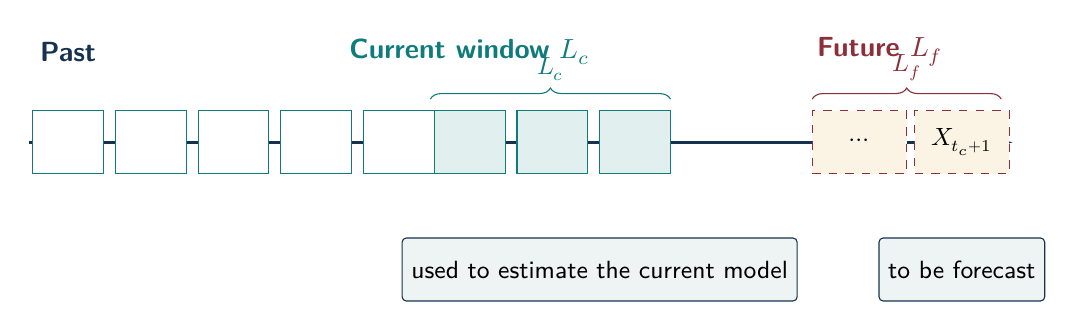
\begin{tikzpicture}[
  >=Latex,
  box/.style={draw=DTNavy, fill=DTMist, rounded corners=1.5pt,
              minimum height=8mm, align=center, font=\sffamily\small},
  obs/.style={draw=DTTeal, fill=white, minimum width=9mm, minimum height=8mm,
              align=center, font=\small},
  future/.style={draw=DTClaret, dashed, fill=DTWarm, minimum width=12mm,
                 minimum height=8mm, align=center, font=\small}
]
  \node[font=\sffamily\bfseries\color{DTNavy}] at (0,1.15) {Past};
  \node[font=\sffamily\bfseries\color{DTTeal}] at (5.1,1.15) {Current window $L_c$};
  \node[font=\sffamily\bfseries\color{DTClaret}] at (10.3,1.15) {Future $L_f$};
  \draw[->, thick, DTNavy] (-0.5,0) -- (12,0);
  \foreach \x in {0,...,4} {
    \node[obs] (h\x) at (\x*1.05,0) {};
  }
  \foreach \x in {0,...,2} {
    \node[obs, draw=DTTeal, fill=DTTeal!12] (c\x) at (5.1+\x*1.05,0) {};
  }
  \node[future] (f1) at (10.05,0) {$\cdots$};
  \node[future] (f2) at (11.35,0) {$X_{t_c+1}$};
  \draw[decorate,decoration={brace,amplitude=4pt},DTTeal]
    (4.6,0.55) -- (7.65,0.55) node[midway,above=3pt,font=\small] {$L_c$};
  \draw[decorate,decoration={brace,amplitude=4pt},DTClaret]
    (9.45,0.55) -- (11.85,0.55) node[midway,above=3pt,font=\small] {$L_f$};
  \node[box, below=8mm of c1, xshift=6mm] {used to estimate the current model};
  \node[box, below=8mm of f2] {to be forecast};
\end{tikzpicture}
\end{center}

\subsection{The formal problem}

The paper calls this \emph{stream forecasting}: given an $L_c$-long window $\mathcal{X}^{c}$, find
time-varying dynamics consisting of trend, seasonality, and diffusion, then forecast at horizon
$L_f$. The output is the matrix at the target time,
$\widehat{X}_{t_c+L_f}\in\mathbb{R}_{+}^{k\times l}$; when evaluating several horizons, the paper
runs each horizon separately and does not claim to emit every intermediate matrix.

\begin{keypoint}
\textbf{Input:} the latest $L_c$ observed matrices, each of size $k\times l$.\\
\textbf{Output:} a forecast at time $t_c+L_f$, plus an interpretable model containing trend,
seasonal, outlier, and diffusion components.\\
\textbf{Constraint:} do not keep the entire stream; each step must cost time independent of the
total number of observed steps.
\end{keypoint}

In the example in Section~\ref{sec:orientation}, $k=2$ (iPhone, Galaxy), $l=2$ (United States,
Vietnam), $L_c=3$ (three observed weeks), and $L_f=1$ for next week. A good model does more than
fit those three weeks; it separates the trend of each pair and represents how interest may spread
between the two places.

\subsection{Why not forecast each series separately?}

We could run a time-series model for every pair $(i,j)$. That ignores two facts:
\begin{itemize}
  \item locations and keywords share latent groups of dynamics; and
  \item the data have multilinear structure, so a small set of factors can describe many pairs at once.
\end{itemize}
D-Tracker finds a small core $\mathcal{W}^{(\mathrm{core})}$ plus location and keyword factors that
reconstruct the whole tensor. This reduces the number of parameters and yields interpretable groups.
The price is a harder optimization problem and the need to test whether those groups are useful.

\begin{plainwords}
Do not picture a tensor as a mysterious block. Picture a stack of tables: one keyword-by-location
table per week. D-Tracker finds a few common table patterns, then mixes them with different weights
for each keyword and location.
\end{plainwords}

\begin{commonmistake}
Two misunderstandings are common. First, a third-order tensor is not ``three physical dimensions'';
its axes are data attributes. Second, the model does not forecast the entire infinite stream at
once: it forecasts $L_f$ steps from the current window, then repeats as new data arrive.
\end{commonmistake}

\subsection{Three questions the model must answer}

The paper evaluates the model with three questions, which also form a reading frame:
\begin{enumerate}
  \item \textbf{Accuracy:} how well does it forecast future values? (MAE, RMSE)
  \item \textbf{Scalability:} how does runtime change as the stream grows?
  \item \textbf{Effectiveness:} does it extract trend, seasonality, and diffusion in an interpretable way?
\end{enumerate}
These are independent: a model can fit well but be unexplainable, or explain beautifully but forecast
poorly. D-Tracker's design is an attempt to balance all three.

\begin{selfcheck}
\begin{enumerate}
  \item For a tensor with $k=8$, $l=50$, and $L_c=104$, how many entries are in one time slice?
  \item Distinguish $t_c$, $L_c$, and $L_f$ in one sentence.
  \item Why does using only the latest window help the model adapt to changing patterns?
\end{enumerate}
\end{selfcheck}

\section{Background: tensors, factorization, and three components}
\label{sec:tensor-primer}

\subsection{Scalar, vector, matrix, tensor}

The word ``tensor'' sounds intimidating, but here it means a \emph{multi-dimensional array}. The
table below contains almost all the background needed for the paper's formulas.

\begin{center}
\small
\begin{tabular}{@{}llll@{}}
  \toprule
  Object & Order & Example notation & How to read it \\
  \midrule
  Scalar & 0 & $x=7$ & one number \\
  Vector & 1 & $\mathbf{w}=(w_1,\ldots,w_k)$ & a list over keywords \\
  Matrix & 2 & $\mathbf{W}\in\mathbb{R}^{k\times l}$ & a keyword $\times$ location table \\
  Tensor & 3 & $\mathcal{X}\in\mathbb{R}^{k\times l\times L_c}$ & a stack of tables over time \\
  \bottomrule
\end{tabular}
\end{center}

Indices follow axis order from left to right. For a third-order tensor, $x_{ij}(t)$ is the entry at
keyword $i$, location $j$, time $t$. If $k=2,l=2,L_c=3$, the tensor has $2\cdot2\cdot3=12$ entries.
\emph{Unfolding} (matricization) turns a tensor into a matrix by grouping axes; unfolding along the
keyword axis, for example, produces a matrix that linear algebra can process. We do not need to
unfold by hand, but we should remember that it only \emph{rearranges} numbers and creates no data.

\subsection{Tucker factorization, intuitively}

Suppose there are $k$ keywords and $l$ locations. Instead of storing every tensor value, assume the
data are generated by a few shared \emph{styles of dynamics}. Let $d_k$ be the number of keyword
groups and $d_l$ the number of location groups, with $d_k\ll k$ and $d_l\ll l$. The trend is then
approximated by
\begin{equation}
  \widehat{\mathcal{X}}_d
  =\mathcal{W}^{(\mathrm{core})}
   \times_{\mathrm{key}}\mathbf{W}^{(\mathrm{key})}
   \times_{\mathrm{loc}}\mathbf{W}^{(\mathrm{loc})},
  \label{eq:tucker-intuition}
\end{equation}
where $\mathcal{W}^{(\mathrm{core})}$ is a small $d_k\times d_l\times L_c$ tensor, and
$\mathbf{W}^{(\mathrm{key})}$ and $\mathbf{W}^{(\mathrm{loc})}$ are non-negative coefficient
matrices of size $d_k\times k$ and $d_l\times l$.

The symbols $\times_{\mathrm{key}},\times_{\mathrm{loc}}$ denote \emph{mode products}. Read
Equation~\eqref{eq:tucker-intuition} as follows: take the small core, spread it over keyword groups
with weights $\mathbf{W}^{(\mathrm{key})}$, then over location groups with
$\mathbf{W}^{(\mathrm{loc})}$. A keyword with a large weight in group 2 receives more of group 2's
dynamics. Non-negative weights cannot flip a dynamics' sign, so ``this group is rising'' remains
readable after mixing.

\begin{keypoint}
Tucker factorization is not arbitrary file compression. It yields a small core containing
\emph{shared dynamics} and factors saying \emph{which members belong to which group}. This is the
bridge between forecasting and interpretation.
\end{keypoint}

\subsection{A \texorpdfstring{$2\times2\times3$}{2x2x3} example and the benefit of compression}

Imagine two keywords, two locations, and three weeks. The raw tensor has 12 numbers. If we assume one
keyword group and one location group ($d_k=d_l=1$), the core has $1\cdot1\cdot3=3$ numbers and the
two factors have $1\cdot2+1\cdot2=4$: seven parameters instead of 12. On real data the gap is much
larger. A Device window has $8\cdot50\cdot104=41{,}600$ entries. With $d_k=3,d_l=2$, the core has
$3\cdot2\cdot104=624$ entries and the factors have $3\cdot8+2\cdot50=124$: about 748 parameters,
less than 2\% of the window.

\begin{plainwords}
Compression here is not about saving disk space. It forces the model to explain tens of thousands of
observations with a few dynamics and a table of ``who belongs to which group''. If the model still
fits, that group structure is a useful hypothesis.
\end{plainwords}

\subsection{Trend, seasonal, and outlier in a tiny series}

The three components in D-Tracker add up to approximately the data:
\begin{equation}
  \mathcal{X}^{c}\approx\widehat{\mathcal{X}}_d
  +\widehat{\mathcal{X}}_s+\widehat{\mathcal{X}}_o.
  \label{eq:decompose-primer}
\end{equation}
Table~\ref{tab:three-components} is a numerical example \textbf{created for this guide}. The
``Observed'' row is exactly the sum of the other three; a dash in the outlier row means zero.

\begin{table}[htbp]
  \centering
  \small
  \caption{Illustrative trend + seasonal + outlier decomposition.}
  \label{tab:three-components}
  \begin{tabular}{lrrrrrrrr}
    \toprule
    Component & Week 1 & 2 & 3 & 4 & 5 & 6 & 7 & 8 \\
    \midrule
    Observed  & 10 & 12 & 15 & 14 & 11 & 13 & 17 & 25 \\
    Trend     & 10 & 11 & 12 & 13 & 14 & 15 & 16 & 17 \\
    Seasonal  &  0 &  1 &  3 &  1 & $-3$ & $-2$ &  1 &  3 \\
    Outlier   &  -- & -- & -- & -- & -- & -- & -- &  5 \\
    \bottomrule
  \end{tabular}
\end{table}

The trend changes relatively smoothly. The seasonal part repeats with a period (a short pattern is
shown here; real data use weekly/annual periods). The outlier part is unusual and assumed
\emph{sparse}: only a few cells are non-zero. This separation prevents a one-off spike from being
mistaken for a permanent change in trend.

\subsection{From decomposition to the paper's question}

We now have three pieces: an observed tensor, a way to compress its trend into a core and factors,
and a three-part decomposition. The paper adds two more ideas:
\begin{itemize}
  \item the trend core does not evolve arbitrarily; it follows a \textbf{reaction--diffusion} system; and
  \item the model is updated as a stream arrives, with the latent structure and switch times selected
        automatically.
\end{itemize}
Section~\ref{sec:reaction-diffusion} explains the first; Section~\ref{sec:model} assembles the full model.

\begin{commonmistake}
Three common errors: (1) treating $\mathcal{W}^{(\mathrm{core})}$ as a shrunken copy of the raw data ---
it is a \emph{latent parameter} that is learned; (2) treating $\mathbf{W}$ as probabilities --- they
are non-negative weights and need not sum to one; (3) assuming the decomposition is unique --- tensor
factorizations are generally only identifiable up to transformations, and the paper solves a
particular optimization problem.
\end{commonmistake}

\begin{selfcheck}
\begin{enumerate}
  \item With $d_k=2$, $d_l=3$, and $L_c=10$, how many entries are in the core?
  \item Explain in one sentence why non-negative factors preserve the direction of a dynamics.
  \item In the three-component table, what would the model misunderstand if the outlier at week 8 were removed?
\end{enumerate}
\end{selfcheck}

\section{Reaction--diffusion: why does interest spread?}
\label{sec:reaction-diffusion}

\subsection{Two reservoirs and one idea}

In chemistry, a substance diffuses from high concentration to low concentration. D-Tracker borrows
that picture for interest: if a keyword receives strong attention in location group $j'$, some of
that attention may flow to group $j$ where activity is lower. The general reaction--diffusion
equation cited by the paper is
\begin{equation}
  \frac{\partial u_i}{\partial t}
  =f(u_i)+\sum_j D\,(u_j-u_i),
  \label{eq:rd-background}
\end{equation}
where $u_i$ is the concentration at position $i$ and $D$ is diffusion strength. The term $f(u_i)$ is
the \textbf{reaction}: local change at a position. The term $\sum_j D(u_j-u_i)$ is
\textbf{diffusion}: it is non-zero only when positions differ, and its sign says whether flow enters
or leaves.

\begin{center}
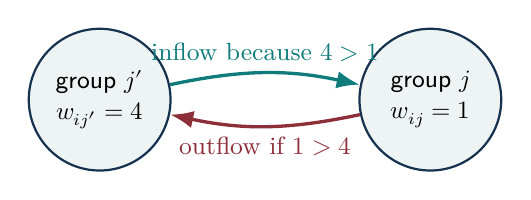
\begin{tikzpicture}[
  >=Latex,
  place/.style={circle, draw=DTNavy, thick, minimum size=18mm, fill=DTMist,
                align=center, font=\sffamily\small},
  flow/.style={->, very thick, DTTeal},
  label/.style={font=\small, align=center}
]
  \node[place] (b) at (0,0) {group $j'$\\$w_{ij'}=4$};
  \node[place] (a) at (4.2,0) {group $j$\\$w_{ij}=1$};
  \draw[flow] (b) to[bend left=12] node[above,label] {inflow because $4>1$} (a);
  \draw[flow, DTClaret] (a) to[bend left=12] node[below,label] {outflow if $1>4$} (b);
\end{tikzpicture}
\end{center}

\subsection{D-Tracker's latent version}

D-Tracker does not impose the equation on every keyword--location pair. It imposes it on a
\emph{latent core} of $d_k\cdot d_l$ dynamics. With $i=1,\ldots,d_k$ indexing keyword groups and
$j=1,\ldots,d_l$ indexing location groups, the paper writes
\begin{equation}
  \frac{dw_{ij}}{dt}
  =a_{ij}w_{ij}
   +\sum_{j'=1}^{d_l} d_{ijj'}\,(w_{ij'}-w_{ij}),
  \qquad 1\leq i\leq d_k,\;1\leq j\leq d_l.
  \label{eq:rd-latent}
\end{equation}
Two parameters need careful reading:
\begin{itemize}
  \item $a_{ij}$ is the \textbf{growth rate}. If $a_{ij}>0$, dynamics $w_{ij}$ tends to rise; if
        $a_{ij}<0$, it tends to fall. This is the ``reaction''.
  \item $d_{ijj'}$ is the \textbf{diffusion strength} from location group $j'$ to group $j$. The
        paper describes $\mathcal{D}\in\mathbb{R}_{+}^{d_k\times d_l\times d_l}$ as non-negative.
        The actual direction also depends on $(w_{ij'}-w_{ij})$: if $w_{ij'}>w_{ij}$, group $j$
        receives; if it is lower, group $j$ loses.
\end{itemize}

Here $w_{ij}$ is the activity of the dynamics for keyword group $i$ and location group $j$. Dynamics
from different keyword groups do not diffuse directly in this sum; they interact through the core
and the multilinear projection in Section~\ref{sec:model}. The full system has $d_k\cdot d_l$
equations with parameters $\mathbf{A}\in\mathbb{R}^{d_k\times d_l}$ and
$\mathcal{D}\in\mathbb{R}_{+}^{d_k\times d_l\times d_l}$.

\begin{keypoint}
$w>0$ makes ``activity'' readable; $a$ says rise or fall; $(w_{j'}-w_j)$ says flow direction; $d$
says how strong the flow is. This is why the model can be interpretable rather than a black-box
forecaster.
\end{keypoint}

\subsection{A concrete one-step calculation}

Suppose a dynamics in group $j$ has $w_j=1$, another dynamics in the same keyword group but location
group $j'$ has $w_{j'}=4$, $a_j=0.1$, and $d_{jj'}=0.5$. Ignoring other groups, the derivative is
\[
  \frac{dw_j}{dt}=0.1\cdot1+0.5\cdot(4-1)=0.1+1.5=1.6.
\]
With an Euler step $\Delta t=1$, the next value is approximately $1+1.6=2.6$. The dynamics is rising
because it has both growth and inflow from a higher group. If $w_{j'}=0$ instead, the diffusion term
becomes $0.5(0-1)=-0.5$: the same strength $d$ but the opposite direction.

\begin{plainwords}
Do not memorize the equation. Read three sentences: ``it grows or shrinks on its own'', ``it is
pulled toward another group'', and ``the larger the gap, the stronger the pull''. All three sentences live
in the two terms of Equation~\eqref{eq:rd-latent}.
\end{plainwords}

\subsection{Connecting back to observations}

The core $w_{ij}$ is latent. To connect it to an observed series $X_{uv}$ for real keyword $u$ and
real location $v$, the paper differentiates the projection and obtains
\begin{equation}
  \frac{dX_{uv}}{dt}
  =\sum_{i=1}^{d_k}\sum_{j=1}^{d_l}
   W^{(\mathrm{key})}_{iu}W^{(\mathrm{loc})}_{jv}
   \underbrace{\left(
     a_{ij}w_{ij}+\sum_{j'=1}^{d_l}d_{ijj'}(w_{ij'}-w_{ij})
   \right)}_{\text{latent reaction--diffusion system}}.
  \label{eq:observed-derivative}
\end{equation}
Read from right to left: the latent system creates $d_k d_l$ dynamics; the non-negative weights
$W^{(\mathrm{key})}_{iu}W^{(\mathrm{loc})}_{jv}$ decide which dynamics contribute to pair $(u,v)$.
Because the weights are non-negative, the projection cannot flip a sign: a rising dynamics still
contributes positively to its series. This is the bridge from the ``small core'' to the ``real series''.

\subsection{Interpretation is not causation}

The reaction--diffusion assumption says that a level gap can create flow. The model learns $a,d$ and
group factors to fit data; it does \emph{not} prove that a rise in the United States caused a rise in
Vietnam. A third factor (a global launch, news, social media) can create the same delayed pattern.
Read the result as a \textbf{structured diffusion hypothesis}, to be checked with domain knowledge and
additional experiments.

\begin{commonmistake}
``$d_{ijj'}>0$ means $j'$ always sends to $j$'' is incomplete. Flow also depends on
$w_{ij'}-w_{ij}$; if $w_{ij'}<w_{ij}$, the term is negative. The paper calls $d$ a strength, not a
fixed direction. Likewise, ``$a>0$'' only describes local tendency, not guaranteed growth forever.
\end{commonmistake}

\begin{selfcheck}
\begin{enumerate}
  \item With $w_j=2,w_{j'}=5,a_j=0,d_{jj'}=0.2$, what is the derivative?
  \item If $a_{ij}<0$ and the diffusion inflow is positive, must the dynamics fall? Why or why not?
  \item Describe a situation with a delay between two places that is not causal diffusion.
\end{enumerate}
\end{selfcheck}

\section{The complete D-Tracker model}
\label{sec:model}

\subsection{Three components added together}

For the current window $\mathcal{X}^{c}$, the paper assumes that observations are approximately the
sum of a trend tensor, a seasonal tensor, and an outlier tensor (paper Eq.~1):
\begin{equation}
  \mathcal{X}^{c}\;\approx\;\widehat{\mathcal{X}}_d
  +\widehat{\mathcal{X}}_s+\widehat{\mathcal{X}}_o,
  \qquad
  \widehat{\mathcal{X}}_d,\widehat{\mathcal{X}}_s,\widehat{\mathcal{X}}_o
  \in\mathbb{R}^{k\times l\times L_c}.
  \label{eq:model-sum}
\end{equation}
The decomposition is not decoration. Each component carries a distinct assumption:
\begin{itemize}
  \item $\widehat{\mathcal{X}}_d$ contains \textbf{trend and diffusion}, the structured changing part;
  \item $\widehat{\mathcal{X}}_s$ contains \textbf{seasonality}, the repeating part;
  \item $\widehat{\mathcal{X}}_o$ contains \textbf{outliers}, assumed sparse and unusual.
\end{itemize}
Without the split, a promotion could be learned as a long-term trend; without the outlier component,
one shock could corrupt every coefficient.

\subsection{Trend: compress a core and project it back}

The trend tensor still has size $k\times l\times L_c$, too large to read directly. The paper
factorizes it into a small core and two factor matrices (paper Eq.~2):
\begin{equation}
  \widehat{\mathcal{X}}_d
  =\mathcal{W}^{(\mathrm{core})}
   \times_{\mathrm{key}}\mathbf{W}^{(\mathrm{key})}
   \times_{\mathrm{loc}}\mathbf{W}^{(\mathrm{loc})},
  \label{eq:trend-factorization}
\end{equation}
with
\[
  \mathcal{W}^{(\mathrm{core})}\in\mathbb{R}^{d_k\times d_l\times L_c},
  \quad
  \mathbf{W}^{(\mathrm{key})}\in\mathbb{R}_{+}^{d_k\times k},
  \quad
  \mathbf{W}^{(\mathrm{loc})}\in\mathbb{R}_{+}^{d_l\times l},
\]
and $d_k\ll k$, $d_l\ll l$. Elementwise, this is
\begin{equation}
  \widehat{x}_{d,uv}(t)
  =\sum_{i=1}^{d_k}\sum_{j=1}^{d_l}
    w^{(\mathrm{core})}_{ij}(t)\,
    W^{(\mathrm{key})}_{iu}W^{(\mathrm{loc})}_{jv}.
  \label{eq:trend-elementwise}
\end{equation}
Each symbol has a concrete meaning: $u$ is a real keyword, $v$ a real location, and $i,j$ latent
groups. If $W^{(\mathrm{key})}_{iu}$ is large, keyword $u$ ``belongs'' to group $i$; if
$W^{(\mathrm{loc})}_{jv}$ is large, location $v$ belongs to group $j$. The core
$w^{(\mathrm{core})}_{ij}(t)$ is the activity curve of that group pair.

\begin{keypoint}
Equation~\eqref{eq:trend-elementwise} is the heart of interpretability: the value for $(u,v)$ is a sum
of latent dynamics, each weighted by how strongly the keyword and location relate to it. Non-negative
weights keep the sum from flipping direction.
\end{keypoint}

\subsection{The core is generated by reaction--diffusion}

The paper does not let $w^{(\mathrm{core})}_{ij}(t)$ vary arbitrarily. It assumes the core is generated
by the system in Equation~\eqref{eq:rd-latent} from Section~\ref{sec:reaction-diffusion}, paper Eq.~3:
\begin{equation}
  \frac{dw_{ij}}{dt}
  =a_{ij}w_{ij}
   +\sum_{j'=1}^{d_l}d_{ijj'}(w_{ij'}-w_{ij}).
  \label{eq:core-ode}
\end{equation}
This is a system of \textbf{ordinary differential equations (ODEs)} in time. Data are observed at
discrete steps (weeks or days), but the model defines continuous-time dynamics and integrates them to
produce a sequence of $L_c$ steps. Positions are discrete (location groups); time in the equation is
continuous.

Let $\theta=\{\mathbf{A},\mathcal{D}\}$ be the system parameters, and let
$w_0\in\mathbb{R}_{+}^{d_k\times d_l}$ be the initial state. The paper writes
$f_\theta(\theta,w_0,L)$ for the function that generates an $L$-long core sequence from $w_0$. The full
trend parameters are therefore
\[
  \theta_d=\{\mathbf{W}^{(\mathrm{key})},\mathbf{W}^{(\mathrm{loc})},\theta\}.
\]
In words, $\theta_d$ contains both ``how the dynamics evolve'' and ``which keywords/locations they
attach to''.

\subsection{Seasonal: a similar factorization}

The seasonal part is compressed too, but without an ODE. The paper factorizes (Eq.~4):
\begin{equation}
  \widehat{\mathcal{X}}_s
  =\mathbf{S}^{(\mathrm{time})}
   \times_{\mathrm{key}}\mathbf{S}^{(\mathrm{key})}
   \times_{\mathrm{loc}}\mathbf{S}^{(\mathrm{loc})},
  \label{eq:seasonal-factorization}
\end{equation}
with $d_s$ seasonal patterns and
\[
  \mathbf{S}^{(\mathrm{time})}\in\mathbb{R}^{d_s\times L_c},
  \quad
  \mathbf{S}^{(\mathrm{key})}\in\mathbb{R}^{d_s\times k},
  \quad
  \mathbf{S}^{(\mathrm{loc})}\in\mathbb{R}^{d_s\times l}.
\]
Elementwise,
\begin{equation}
  \widehat{x}_{s,uv}(t)
  =\sum_{r=1}^{d_s}
    S^{(\mathrm{time})}_{r,t}S^{(\mathrm{key})}_{r,u}S^{(\mathrm{loc})}_{r,v}.
  \label{eq:seasonal-elementwise}
\end{equation}
Each $r$ is a seasonal ``template'' over time; the other factors say how strong it is for each
keyword and location. This is a PARAFAC factorization: each pattern is a rank-one sum of three
vectors. The paper does not state that seasonal factors must be non-negative like the trend
$\mathbf{W}$, so this guide does not add that constraint.

\subsection{Outliers: sparse, not all noise}

The outlier tensor $\widehat{\mathcal{X}}_o$ is assumed \emph{sparse}: most entries are zero, retaining
only unusual values not explained by trend and seasonality. During optimization, the paper takes the
residual $\mathcal{X}^{c}-\widehat{\mathcal{X}}_d-\widehat{\mathcal{X}}_s$ and keeps entries only
when they reduce the total MDL cost. ``Outlier'' is therefore a structured component, not a label for
``bad data''.

\subsection{Parameter sets and multiple regimes}

A single model is packaged as
\[
  \Theta=\{\theta_d,\theta_s,\widehat{\mathcal{X}}_o\},
  \qquad
  \theta_s=\{\mathbf{S}^{(\mathrm{time})},\mathbf{S}^{(\mathrm{key})},
             \mathbf{S}^{(\mathrm{loc})}\}.
\]
When patterns change, one $\Theta$ is insufficient. The paper allows $N$ models:
\[
  \mathcal{F}=\{\Theta_1,\Theta_2,\ldots,\Theta_N\}.
\]
Each $\Theta_n$ describes a relatively stable period; $N$ and switch times are selected automatically
by MDL in Section~\ref{sec:mdl-streaming}, not split by eye. Thus, in a plot such as
Figure~\ref{fig:preview}(a), the dotted lines are not data events; they are model boundaries.

\begin{center}
\small
\begin{tabular}{@{}p{0.24\linewidth}p{0.68\linewidth}@{}}
  \toprule
  Parameter & What it contains \\
  \midrule
  $\theta$ & $\mathbf{A}$ (growth) and $\mathcal{D}$ (diffusion) of the latent system. \\
  $\theta_d$ & Trend core, keyword/location factors, and $\theta$. \\
  $\theta_s$ & Seasonal patterns and keyword/location factors. \\
  $\Theta$ & One complete model: trend, seasonality, and outliers. \\
  $\mathcal{F}$ & A collection of $\Theta$ models for different stream periods. \\
  \bottomrule
\end{tabular}
\end{center}

\subsection{Reading one dynamics from core to raw data}

Suppose the model learns $d_k=3$ keyword groups and $d_l=2$ location groups. To understand
``Dynamics \#1 of Group 1'' in Figure~\ref{fig:preview}(b), follow four steps:
\begin{enumerate}
  \item Look at the core curve: is the dynamics rising, falling, or changing direction?
  \item Look at the corresponding keyword-factor column: which keywords have high weights? In the
        2019--2021 example, the paper associates ``iPhone'' strongly with Dynamics \#1.
  \item Look at the location-factor row: which groups have high weights? The paper describes Group~1
        as the United States, Europe, and China, and Group~2 as the rest of the world.
  \item Inspect $d_{ijj'}$ and the sign of $(w_{ij'}-w_{ij})$ to read the direction. The paper says
        Dynamics \#1 spreads from Group~1 to Group~2, i.e.\ interest in ``iPhone'' diffused from the
        leading regions to the rest of the world in that period.
\end{enumerate}
This is \emph{model-based interpretation}, not a human-provided label. The name ``Group 1'' only gains
meaning after the factors are learned; it need not match a continent or language.

\begin{plainwords}
To read the result, picture three layers: the small core says ``what is happening'', the factor
rows/columns say ``where and for which keyword'', and the diffusion arrows say ``from which group to
which group''. You do not need to stare at the raw tensor.
\end{plainwords}

\begin{commonmistake}
A common error is to treat $d_l\ll k$ in the paper's prose as a real constraint. The shape of
$\mathbf{W}^{(\mathrm{loc})}$ is $d_l\times l$, and the intent is to reduce the number of location
groups, so this guide uses $d_k\ll k$, $d_l\ll l$. This is a likely typo in the paper, surfaced rather
than copied silently. Another error is to conflate $\Theta$ and $\mathcal{F}$: $\mathcal{F}$ is a
\emph{set} of models for different periods.
\end{commonmistake}

\begin{selfcheck}
\begin{enumerate}
  \item Write the shapes of the four objects in Equation~\eqref{eq:trend-factorization}.
  \item Distinguish $\theta$, $\theta_d$, $\Theta$, and $\mathcal{F}$ in one sentence each.
  \item Why does seasonality not need a reaction--diffusion ODE? Which assumption differs from trend?
  \item If $N=1$ for the whole stream, what is the model assuming?
\end{enumerate}
\end{selfcheck}

\section{Parameter estimation: the ALS loop}
\label{sec:estimation}

\subsection{Optimization, intuitively}

We have data $\mathcal{X}^{c}$ and a model with several blocks: a trend core, a reaction--diffusion
system, keyword/location factors, seasonal factors, and outliers. Optimizing everything at once is
both nonlinear and high-dimensional. The paper uses \textbf{ALS} (alternating least squares): hold
most parameters fixed, update one block, and repeat until convergence.

\begin{keypoint}
ALS means ``fix everything else, then solve one part as well as possible''. It does not guarantee a
global optimum for a non-convex problem; the paper uses it as a practical procedure and reports
empirical results.
\end{keypoint}

For readability, call the squared reconstruction error of a model
\begin{equation}
  \mathcal{L}(\Theta)
  =\left\|\mathcal{X}^{c}
    -\widehat{\mathcal{X}}_d-\widehat{\mathcal{X}}_s-\widehat{\mathcal{X}}_o
   \right\|_F^2.
  \label{eq:als-loss}
\end{equation}
The paper does not name this symbol in Section 4.1, but every update below reduces this error (or the
MDL cost at the outlier step). The Frobenius norm $\|\cdot\|_F$ is the square root of the sum of
squared entries, a measure of how far the model is from the data.

\subsection{Initialization: STL, PARAFAC, and NTD}

ModelEstimation needs a starting point. The paper describes three initialization steps:
\begin{enumerate}
  \item Apply \textbf{STL} (seasonal-trend decomposition using LOESS) to the current window, splitting
        it into trend, seasonal, and residual. STL is a classical statistical method suited to
        seasonal series; it provides initial approximations of $\widehat{\mathcal{X}}_d$ and
        $\widehat{\mathcal{X}}_s$.
  \item Factorize $\widehat{\mathcal{X}}_s$ with \textbf{PARAFAC} to initialize
        $\mathbf{S}^{(\mathrm{time})},\mathbf{S}^{(\mathrm{key})},\mathbf{S}^{(\mathrm{loc})}$.
  \item Apply \textbf{Nonnegative Tucker Decomposition (NTD)} to $\widehat{\mathcal{X}}_d$ to
        initialize $\mathbf{W}^{(\mathrm{key})},\mathbf{W}^{(\mathrm{loc})}$.
\end{enumerate}
The outlier tensor starts at zero: initially, no outlier is assumed. Initialization is not a minor
detail; it affects whether ALS lands in a poor local solution, and the paper documents it in
Appendix A.1.

\subsection{Updating the reaction--diffusion system}

Holding $\mathbf{W}^{(\mathrm{key})},\mathbf{W}^{(\mathrm{loc})}$ and the other components fixed, the
paper solves the nonlinear least-squares problem
\begin{equation}
  \{\theta,w_0\}
  =\arg\min_{\theta',w_0'}
   \left\|
     \mathcal{X}^{c}-\widehat{\mathcal{X}}_s-\widehat{\mathcal{X}}_o
     -f_\theta(\theta',w_0',L_c)
       \times_{\mathrm{key}}\mathbf{W}^{(\mathrm{key})}
       \times_{\mathrm{loc}}\mathbf{W}^{(\mathrm{loc})}
   \right\|_F^2,
  \label{eq:lm-estimation}
\end{equation}
which is Eq.~(5) in the paper. The symbol $\arg\min$ means ``choose parameters that make the expression
smallest''. Because $f_\theta$ contains the ODE solution, its derivative with respect to $\theta$ has no
simple closed form. The paper uses \textbf{Levenberg--Marquardt (LM)}, a numerical nonlinear
least-squares method, to update $\mathbf{A},\mathcal{D}$ and the initial state $w_0$ jointly.

We need not implement LM to understand the paper, but should remember three things: (i) this is the
expensive step; (ii) it needs an ODE solver; (iii) its result depends on initialization and may be a
local optimum.

\subsection{Updating trend factors by multiplicative updates}

Once the core $\mathcal{W}^{(\mathrm{core})}$ is available, the paper updates each trend factor. With
``mode'' being key or loc, define
\begin{align}
  \mathbf{P}^{(\mathrm{mode})}
  &=\max\!\left(\epsilon,\;
    \mathbf{X}_d^{(\mathrm{mode})}\cdot\mathbf{G}^{(\mathrm{mode})}
   \right), \label{eq:w-p}\\
  \mathbf{Q}^{(\mathrm{mode})}
  &=\max\!\left(\epsilon,\;
    \mathbf{W}^{(\mathrm{mode})}\cdot\mathbf{G}^{(\mathrm{mode})}
    \cdot(\mathbf{G}^{(\mathrm{mode})})^{\mathsf T}
   \right), \label{eq:w-q}\\
  \mathbf{W}^{(\mathrm{mode})}
  &\leftarrow
    \mathbf{W}^{(\mathrm{mode})}
    \otimes\mathbf{P}^{(\mathrm{mode})}
    \oslash\mathbf{Q}^{(\mathrm{mode})}.
  \label{eq:multiplicative}
\end{align}
This is Eq.~(6) in the paper. Here:
\begin{itemize}
  \item $\mathbf{X}_d^{(\mathrm{mode})}$ is the residual tensor
        $\mathcal{X}^{c}-\widehat{\mathcal{X}}_s-\widehat{\mathcal{X}}_o$, \emph{unfolded} along
        the mode (Eq.~7);
  \item $\mathbf{G}^{(\mathrm{mode})}$ is the remaining projection, also unfolded;
  \item $\otimes$ is elementwise (Hadamard) product and $\oslash$ elementwise division;
  \item $\epsilon$ is a tiny positive constant that prevents division by zero.
\end{itemize}
Since $\mathbf{W}$ starts non-negative and the update only multiplies/divides positive quantities, it
stays non-negative. This is why ``multiplicative'' matters: it optimizes while preserving the
constraint.

\begin{plainwords}
Equation~(6) looks heavy, but the idea is: compare the missing data with what the model predicts, then
nudge each weight up or down by a ratio. No unrestricted subtraction can push a weight below zero.
\end{plainwords}

\subsection{Updating seasonal factors}

For seasonality, the paper holds the other components fixed and uses a closed-form ALS step. For each
mode in $\{\mathrm{time},\mathrm{key},\mathrm{loc}\}$, define
\begin{align}
  \mathbf{U}^{(\mathrm{mode})}
  &=\odot_{i\neq\mathrm{mode}}\mathbf{S}^{(i)},&
  \mathbf{V}^{(\mathrm{mode})}
  &=\otimes_{i\neq\mathrm{mode}}
    (\mathbf{S}^{(i)})^{\mathsf T}\mathbf{S}^{(i)},\\
  \mathbf{S}^{(\mathrm{mode})}
  &\leftarrow
    \mathbf{X}_s^{(\mathrm{mode})}
    \mathbf{U}^{(\mathrm{mode})}
    (\mathbf{V}^{(\mathrm{mode})})^{\dagger}.
  \label{eq:seasonal-update}
\end{align}
This is Eq.~(8); $\odot$ and $\otimes$ denote Khatri--Rao and elementwise products, $\dagger$ is the
Moore--Penrose pseudoinverse, and $\mathbf{X}_s^{(\mathrm{mode})}$ is the residual
$\mathcal{X}^{c}-\widehat{\mathcal{X}}_d-\widehat{\mathcal{X}}_o$ unfolded along the mode (Eq.~9).
Intuitively, it is the linear least-squares solution while the other two modes are fixed; the proof is
not repeated here.

\subsection{Updating outliers by sparsification}

After updating trend and seasonality, the remaining residual is
$\mathcal{R}=\mathcal{X}^{c}-\widehat{\mathcal{X}}_d-\widehat{\mathcal{X}}_s$. The paper does not use
a manual rule such as ``larger than 3 is an outlier''. It considers each residual entry and decides
whether to keep it or set it to zero so that total MDL cost is smallest. The cost is detailed in
Section~\ref{sec:mdl-streaming}; here, the result is a sparse tensor.

\subsection{The full loop and complexity}

\begin{tcolorbox}[enhanced,breakable,colback=white,colframe=DTNavy,arc=1.5mm,
  title={\sffamily\bfseries Algorithm 2 --- ModelEstimation (summary)},fonttitle=\small,
  coltitle=white,colbacktitle=DTNavy,left=3mm,right=3mm,top=2mm,bottom=2mm]
\textbf{Input:} $\mathcal{X}^{c},d_k,d_l,d_s$.\quad
\textbf{Output:} $\Theta=\{\theta_d,\theta_s,\widehat{\mathcal{X}}_o\}$.
\begin{enumerate}[leftmargin=1.5em]
  \item Initialize $\theta_d,\theta_s$ with STL + PARAFAC + NTD; set $\widehat{\mathcal{X}}_o=0$.
  \item \textbf{repeat}
  \item \quad Update $\theta=\{\mathbf{A},\mathcal{D}\}$ and $w_0$ with LM (Eq.~5).
  \item \quad Generate $\mathcal{W}^{(\mathrm{core})}=f_\theta(\theta,w_0,L_c)$.
  \item \quad Update $\mathbf{W}^{(\mathrm{key})},\mathbf{W}^{(\mathrm{loc})}$ (Eq.~6).
  \item \quad Update $\mathbf{S}^{(\mathrm{time})},\mathbf{S}^{(\mathrm{key})},
        \mathbf{S}^{(\mathrm{loc})}$ (Eq.~8).
  \item \quad Sparsify the residual to update $\widehat{\mathcal{X}}_o$.
  \item \textbf{until} convergence.
\end{enumerate}
\end{tcolorbox}

Lemma~1 (in §4.1; the HTML labels it Lemma~4.1) states that ModelEstimation takes time
\[
  O(d_k d_l^2+kd_k+ld_l).
\]
The term $d_k d_l^2$ comes from the reaction--diffusion parameters and the rest from updating the two
factor matrices. The expression omits ALS iterations, ODE solving, seasonal updates, and outlier
updates. Read it as the complexity of \emph{one main update pass} as presented by the paper, not a
guarantee for the whole pipeline.

\begin{commonmistake}
``Convergence'' does not mean a global optimum. ALS on a non-convex problem can stop at a local
solution; the paper does not prove global optimality. Also, $\epsilon$ is not a model parameter to
learn; it only guards a division.
\end{commonmistake}

\begin{selfcheck}
\begin{enumerate}
  \item Why does the $\theta$ update need LM instead of a closed-form solution?
  \item Why does $\mathbf{W}\otimes\mathbf{P}\oslash\mathbf{Q}$ preserve non-negativity?
  \item Name the three initialization methods and what each initializes.
  \item Which costs are omitted from $O(d_kd_l^2+kd_k+ld_l)$?
\end{enumerate}
\end{selfcheck}

\section{MDL, structure selection, and streaming}
\label{sec:mdl-streaming}

\subsection{MDL through an everyday picture}

Imagine sending a data file to a colleague over a very slow channel. You can send the raw file, or a
``formula describing the file'' plus the part that does not match the formula. If the formula is too
simple, the leftover corrections are huge. If it is too complex, the formula itself is long.
\textbf{Minimum Description Length} (MDL) chooses the description with the smallest \emph{total
number of bits}:
\begin{equation}
  \bigl\langle \mathcal{X};\mathcal{F}\bigr\rangle
  =\bigl\langle \mathcal{F}\bigr\rangle
   +\bigl\langle \mathcal{X}\mid\mathcal{F}\bigr\rangle.
  \label{eq:mdl-total}
\end{equation}
This is Eq.~(10) in the paper. The first term is the model description cost; the second is the cost of
encoding the data given the model. A good model is not a perfect fit, but one that explains much data
with few bits.

\begin{keypoint}
MDL balances \textbf{fit} and \textbf{complexity}. It is used to choose latent dimensions, decide
which outliers to keep, and decide whether to add a new regime. This is why the paper calls the method
``automatic''.
\end{keypoint}

\subsection{Model description cost}

For each model $\Theta$, the paper charges for non-zero parameters. Let $|\cdot|$ denote the number of
non-zero entries, $c_F=32$ the bits per float, and $\log^*$ the universal code length for an integer.
The formulas follow one pattern:
\begin{align}
  \bigl\langle\mathcal{F}\bigr\rangle
  &=\sum_{\Theta\in\mathcal{F}}\bigl\langle\Theta\bigr\rangle,
  &
  \bigl\langle\Theta\bigr\rangle
  &=\bigl\langle\theta_d\bigr\rangle
   +\bigl\langle\theta_s\bigr\rangle
   +\bigl\langle\widehat{\mathcal{X}}_o\bigr\rangle,
  \label{eq:model-cost}\\
  \bigl\langle\mathbf{W}^{(\mathrm{key})}\bigr\rangle
  &=|\mathbf{W}^{(\mathrm{key})}|
    \bigl(\log d_k+\log k+c_F\bigr)
    +\log^*|\mathbf{W}^{(\mathrm{key})}|,
  \label{eq:cost-wkey}\\
  \bigl\langle\mathbf{W}^{(\mathrm{loc})}\bigr\rangle
  &=|\mathbf{W}^{(\mathrm{loc})}|
    \bigl(\log d_l+\log l+c_F\bigr)
    +\log^*|\mathbf{W}^{(\mathrm{loc})}|,\\
  \bigl\langle\theta\bigr\rangle
  &=\bigl\langle\mathbf{A}\bigr\rangle
   +\bigl\langle\mathcal{D}\bigr\rangle,\\
  \bigl\langle\mathbf{A}\bigr\rangle
  &=|\mathbf{A}|\bigl(\log d_k+\log d_l+c_F\bigr)
    +\log^*|\mathbf{A}|,\\
  \bigl\langle\mathcal{D}\bigr\rangle
  &=|\mathcal{D}|\bigl(\log d_k+2\log d_l+c_F\bigr)
    +\log^*|\mathcal{D}|.
  \label{eq:cost-theta}
\end{align}
Seasonal factors and outliers have analogous costs:
\begin{align}
  \bigl\langle\mathbf{S}^{(\mathrm{time})}\bigr\rangle
  &=|\mathbf{S}^{(\mathrm{time})}|
    \bigl(\log d_s+\log L_c+c_F\bigr)
    +\log^*|\mathbf{S}^{(\mathrm{time})}|,\\
  \bigl\langle\mathbf{S}^{(\mathrm{key})}\bigr\rangle
  &=|\mathbf{S}^{(\mathrm{key})}|
    \bigl(\log d_s+\log k+c_F\bigr)
    +\log^*|\mathbf{S}^{(\mathrm{key})}|,\\
  \bigl\langle\mathbf{S}^{(\mathrm{loc})}\bigr\rangle
  &=|\mathbf{S}^{(\mathrm{loc})}|
    \bigl(\log d_s+\log l+c_F\bigr)
    +\log^*|\mathbf{S}^{(\mathrm{loc})}|,\\
  \bigl\langle\widehat{\mathcal{X}}_o\bigr\rangle
  &=|\widehat{\mathcal{X}}_o|
    \bigl(\log n+\log k+\log l+c_F\bigr)
    +\log^*|\widehat{\mathcal{X}}_o|.
  \label{eq:cost-outlier}
\end{align}
You need not memorize each line. What matters: cost grows with the number of non-zero entries and axis
sizes, so increasing $d_k,d_l,d_s$ makes the model more expensive, and adding outliers also costs bits.
The symbol $n$ in the outlier cost is not redefined at the formula; the paper uses it as the stream
length/total size. This is an ambiguity, so this guide preserves the formula and flags it instead of
assigning a confident meaning.

\subsection{Data encoding cost}

The remaining term describes the data under the model. The paper uses Huffman coding and a Gaussian
noise model with mean $\mu$ and variance $\sigma^2$:
\begin{equation}
  \bigl\langle\mathcal{X}\mid\mathcal{F}\bigr\rangle
  =\sum_{x\in\mathcal{X}}
   -\log_2 p_{\mu,\sigma}
   \bigl(x-\widehat{x}_d-\widehat{x}_s-\widehat{x}_o\bigr).
  \label{eq:data-cost}
\end{equation}
This is the unnumbered equation immediately after Eq.~(10). Intuitively, if the residual
$x-\widehat{x}_d-\widehat{x}_s-\widehat{x}_o$ is small and consistent with expected noise, it costs few
bits; an unusually large residual costs many bits. The model must therefore fit without turning every
small fluctuation into a parameter.

\begin{plainwords}
MDL does not ask ``which model fits best?''. It asks ``which model gives the shortest description of
both the model and the data?''. An over-large model can fit perfectly but describe itself at length; an
over-small model is compact but leaves a long residual. The optimal structure is the balance point.
\end{plainwords}

\subsection{How are outliers and dimensions selected?}

For outliers, the paper tries setting each residual entry to zero and keeps the change if total cost
falls. This is principled sparsification, not a hand-picked threshold.

For dimensions, Algorithm~4 (\textsc{RankUpdate}) tries configurations that change one rank by one:
$(d_k-1,d_l,d_s)$, $(d_k+1,d_l,d_s)$, $(d_k,d_l-1,d_s)$, $(d_k,d_l+1,d_s)$,
$(d_k,d_l,d_s-1)$, $(d_k,d_l,d_s+1)$. Each candidate is re-estimated and the lowest-cost structure is
kept. In the paper's HTML/PDF listing, the candidate list repeats $(d_k,d_l+1,d_s)$ and omits
$(d_k+1,d_l,d_s)$; this is very likely a presentation error. This guide uses the complete
``change one rank'' idea and states the discrepancy.

\subsection{ModelUpdate: add, keep, or switch regime?}

Algorithm~3 compares the total cost of adding a candidate $\Theta'$ to the model set $\mathcal{F}$ with
the cost without it. If adding lowers cost, the candidate is accepted; otherwise the old model remains.
After acceptance, RankUpdate may adjust $d_k,d_l,d_s$.

\begin{center}
\resizebox{\textwidth}{!}{%
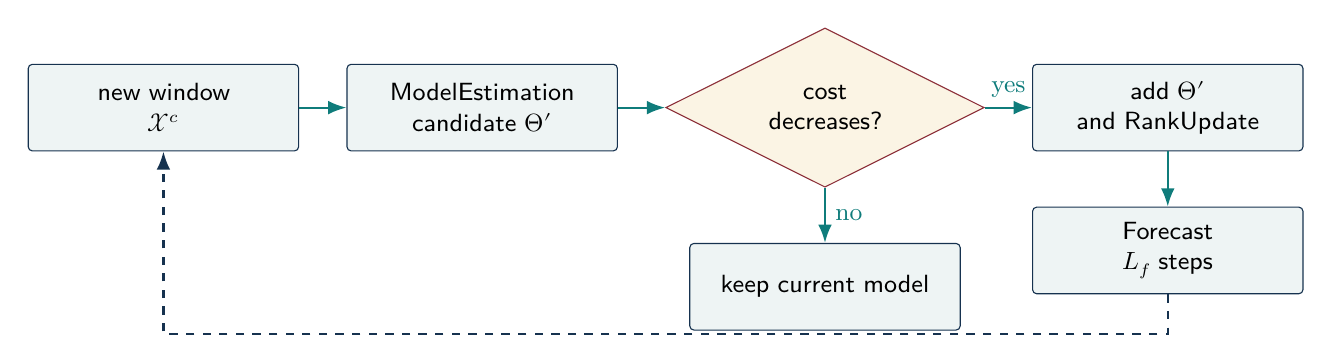
\begin{tikzpicture}[
  >=Latex,
  node distance=6mm and 6mm,
  stage/.style={draw=DTNavy, rounded corners=1.5pt, fill=DTMist,
    text width=3.2cm, minimum height=11mm, align=center, font=\sffamily\small},
  decision/.style={diamond, draw=DTClaret, fill=DTWarm, aspect=2.0,
    text width=2.2cm, align=center, font=\sffamily\small},
  arrow/.style={->, thick, DTTeal}
]
  \node[stage] (x) {new window\\$\mathcal{X}^{c}$};
  \node[stage, right=of x] (est) {ModelEstimation\\candidate $\Theta'$};
  \node[decision, right=of est] (cost) {cost\\decreases?};
  \node[stage, right=of cost] (add) {add $\Theta'$\\and RankUpdate};
  \node[stage, below=7mm of cost] (keep) {keep current model};
  \node[stage, below=7mm of add] (fc) {Forecast\\$L_f$ steps};
  \draw[arrow] (x) -- (est);
  \draw[arrow] (est) -- (cost);
  \draw[arrow] (cost) -- node[above,font=\small]{yes} (add);
  \draw[arrow] (cost) -- node[right,font=\small]{no} (keep);
  \draw[arrow] (add) -- (fc);
  \draw[arrow, dashed, DTNavy] (fc.south) -- ++(0,-0.5) -| (x.south);
\end{tikzpicture}%
}
\end{center}

\subsection{The full streaming algorithm}

Algorithm~1 initializes on the first window, sets $\mathcal{F}=\{\Theta\}$, and then for each time
$t_c$:
\begin{enumerate}
  \item take the current window $\mathcal{X}^{c}$;
  \item run ModelEstimation to obtain candidate $\Theta'$;
  \item run ModelUpdate to add/keep and update ranks;
  \item forecast $L_f$ steps using $\mathcal{F}$;
  \item advance to the next time point.
\end{enumerate}

\begin{keypoint}
Per-step cost does not depend on total stream length because step 1 always takes exactly $L_c$ slices.
The set $\mathcal{F}$ may grow when a new regime appears, and RankUpdate creates runtime spikes, but no
loop touches the entire history. This is the precise meaning of scalability in the paper.
\end{keypoint}

\subsection{Forecast and what the paper does not state}

Algorithm~1 calls
$\widehat{\mathcal{X}}_{t_c+L_f}=\mathrm{Forecast}(\mathcal{F})$, but the main text does not spell out
the Forecast formula. This guide therefore states only what is certain: forecasting uses the active
model in $\mathcal{F}$, and the trend can be extrapolated from the reaction--diffusion system. It does
\emph{not} invent a detailed recurrence for seasonal/outlier terms. For exact reproduction, read the
authors' code or implementation appendix.

\subsection{What does ``parameter-free'' mean?}

The paper says D-Tracker requires no parameter tuning. Read this in context: the user does not manually
choose $d_k,d_l,d_s$ or regime switch times; MDL selects them. Technical choices still exist, such as
the ODE solver, ALS iteration count, convergence tolerance, and the initialization search over
$d_k,d_l\in[2,4]$, $d_s\in[0,4]$ used in the experiments. ``No hyperparameters'' does not mean ``no
numerical settings whatsoever''.

\begin{commonmistake}
Do not say ``MDL always finds the true model''. MDL optimizes a coding criterion; if the noise
assumption is wrong, or reality is more complex than the model family, the MDL-optimal model can still
forecast poorly. It also does not replace causal validation of diffusion arrows.
\end{commonmistake}

\begin{selfcheck}
\begin{enumerate}
  \item If $d_k$ increases, which part of MDL rises, and which part may fall?
  \item Why are outliers not selected by a fixed threshold?
  \item What does ModelUpdate do when a candidate does not reduce total cost?
  \item Explain in one sentence why per-step runtime does not grow with stream length.
\end{enumerate}
\end{selfcheck}

\section{Experiments: reading the results without overclaiming}
\label{sec:experiments}

\subsection{Three empirical questions}

The paper evaluates D-Tracker with three questions:
\begin{description}[leftmargin=1.8em,style=nextline]
  \item[Q1 --- Accuracy.] How accurately does it forecast compared with strong methods?
  \item[Q2 --- Scalability.] How does runtime change as the stream grows?
  \item[Q3 --- Effectiveness.] Does it extract trend, seasonality, and diffusion in a readable way?
\end{description}
Do not merge these questions. A model can win MAE without explaining diffusion; a beautiful diffusion
map does not prove good forecasting. Read the section as three separate views of one model.

\subsection{Data}

The paper uses five GoogleTrends streams and one COVID-19 stream. Table~\ref{tab:datasets} is copied
from paper Table~4; shapes are ordered (time, keywords, locations).

\begin{table}[htbp]
  \centering
  \small
  \caption{The six datasets in the paper (paper Table~4). Keyword names are preserved.}
  \label{tab:datasets}
  \begin{tabular}{@{}cl>{\raggedright\arraybackslash}p{5.6cm}c@{}}
    \toprule
    ID & Dataset & Keywords & Shape \\
    \midrule
    1 & Device & Apple Watch, Fitbit, Galaxy, Google Pixel, Macbook, Xperia, iPad, iPhone & $(676,8,50)$ \\
    2 & Pythonlib & matplotlib, numpy, pandas, pytorch, scipy, sklearn, tensorflow & $(676,7,50)$ \\
    3 & VoD & Apple TV, DAZN, HBO, Prime Video, hulu, netflix, youtube & $(676,7,50)$ \\
    4 & Chatapp & facebook, instagram, slack, snapchat, tiktok, twitter, viber, whatsapp & $(676,8,50)$ \\
    5 & Language & CSS, HTML, Java, JavaScript, PHP, Ruby, SQL, python, swift & $(676,9,50)$ \\
    6 & Covid-19 & new infected, new deceased & $(990,2,50)$ \\
    \bottomrule
  \end{tabular}
\end{table}

GoogleTrends is weekly data from 2010 to 2022. Covid-19 is daily data from January 2020 to September
2022. Everything is min--max normalized to $[0,1]$. There is a small inconsistency in the paper: the
prose says 48 countries, while paper Table~4 uses 50 locations. This guide preserves both and does not
``fix'' either number.

\subsection{Forecast setup}

For GoogleTrends, the current window is $L_c=104$ weeks (two years), and the horizon is
$L_f\in\{13,26,39\}$ weeks (3, 6, 9 months). For Covid-19, $L_c=56$ days (eight weeks), and
$L_f\in\{7,14,21\}$ days, described as 1, 2, 3 weeks in the results. Baselines are DISMO, FluxCube,
PatchTST, Autoformer, DeepAR, LaST, and CoST. Training and tuning details are in Appendix~B.1; D-Tracker
updates a fixed-window model instead of retraining from the entire history at every step.

\subsection{MAE and RMSE: get the direction right}

For $n$ forecasts, let $y_i$ be the truth and $\hat y_i$ the prediction:
\[
  \mathrm{MAE}=\frac1n\sum_{i=1}^n|y_i-\hat y_i|,
  \qquad
  \mathrm{RMSE}=\sqrt{\frac1n\sum_{i=1}^n(y_i-\hat y_i)^2}.
\]
Both are \textbf{better when smaller}. MAE measures average error; RMSE punishes large errors more
strongly. An illustrative pair of errors $-0.04$ and $+0.08$ gives MAE $=0.06$ and
RMSE $=\sqrt{(0.0016+0.0064)/2}\approx0.063$. This is a made-up metric example, not a paper result.

\begin{commonmistake}
Do not compare a paper Table~3 MAE of $0.84$ directly with an unnormalized raw value of $0.84$. The table
header specifies units of $\times10^{-2}$; this guide preserves the printed values and does not convert
them silently. State the unit whenever you quote them.
\end{commonmistake}

\subsection{Q1: accuracy}

Table~\ref{tab:dtracker-mae} copies only D-Tracker rows from paper Table~3, not baselines. The paper
concludes that D-Tracker has the best MAE on \emph{all} datasets and greatly reduces RMSE, while also
acknowledging that some RMSE values are comparable because RMSE is sensitive to large errors. Both
statements belong together.

\begin{table}[htbp]
  \centering
  \scriptsize
  \caption{D-Tracker MAE and RMSE values from paper Table~3, exactly as printed (table units:
  $\times10^{-2}$). Columns 1/2/3 are the three $L_f$ horizons in the dataset name.}
  \label{tab:dtracker-mae}
  \begin{tabular}{@{}lccccccc@{}}
    \toprule
    & & \multicolumn{3}{c}{MAE} & \multicolumn{3}{c}{RMSE} \\
    \cmidrule(lr){3-5}\cmidrule(lr){6-8}
    Dataset & $L_f$ & 1 & 2 & 3 & 1 & 2 & 3 \\
    \midrule
    Device & 13/26/39 & 0.84 & 0.90 & 0.97 & 1.82 & 1.95 & 2.18 \\
    Pythonlib & 13/26/39 & 0.27 & 0.32 & 0.37 & 1.42 & 1.54 & 1.78 \\
    VoD & 13/26/39 & 0.53 & 0.59 & 0.63 & 1.58 & 1.83 & 2.02 \\
    Chatapp & 13/26/39 & 0.28 & 0.34 & 0.41 & 0.83 & 1.01 & 1.24 \\
    Language & 13/26/39 & 0.31 & 0.35 & 0.40 & 0.97 & 1.14 & 1.32 \\
    Covid-19 & 7/14/21 & 0.47 & 0.70 & 0.98 & 1.40 & 2.42 & 3.65 \\
    \bottomrule
  \end{tabular}
\end{table}

Two headline numbers appear in the final bullet of §1: ``up to 57\% improvement'' and ``up to
8.0$\times$ faster''. The paper does
not state the denominator of 57\% in that sentence, so this guide writes ``the paper reports up to
57\%'', without recomputing it or assigning it to a metric. Likewise, 8.0$\times$ is a result on the
paper's hardware, not a universal constant.

\subsection{Ablation: which component contributes?}

\begin{figure}[htbp]
  \centering
  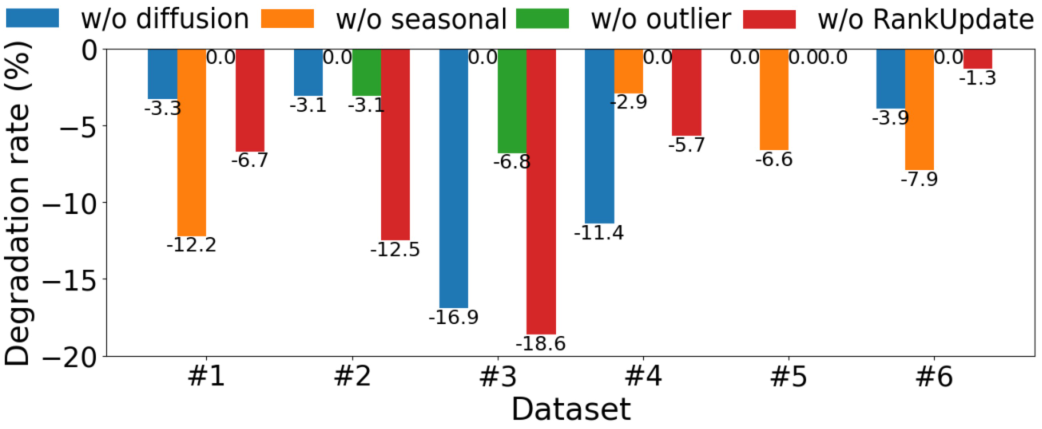
\includegraphics[width=0.95\linewidth]{figures/drop_rate.png}
  \caption{Ablation study. Higher bars represent larger degradation when a component is removed.
  Source: Higashiguchi et al. (2025), arXiv:2505.00242v1, Figure~3; author-owned figure, CC BY 4.0.}
  \label{fig:ablation}
\end{figure}

Figure~\ref{fig:ablation} removes diffusion, seasonal, outlier, and RankUpdate in turn. Degradation
rates are measured at a horizon of 26 weeks (GoogleTrends) or 14 days (Covid-19). The paper reports:
\begin{itemize}
  \item seasonal terms improve datasets with strong seasonality such as Device, Language, and Covid-19;
  \item diffusion improves VoD and Chatapp noticeably;
  \item outliers help some datasets by filtering abrupt changes;
  \item RankUpdate helps the model adapt when the optimal dimension changes.
\end{itemize}
The exceptions matter too. In Language, diffusion does not improve accuracy; the paper suggests there
may be little cross-country diffusion for programming languages. In datasets with few seasonal patterns
or outliers, those components may not help. A model that wins on average does not imply every module
is useful everywhere.

\subsection{Q2: scalability}

\begin{figure}[htbp]
  \centering
  \begin{subfigure}[t]{0.49\linewidth}
    \centering
    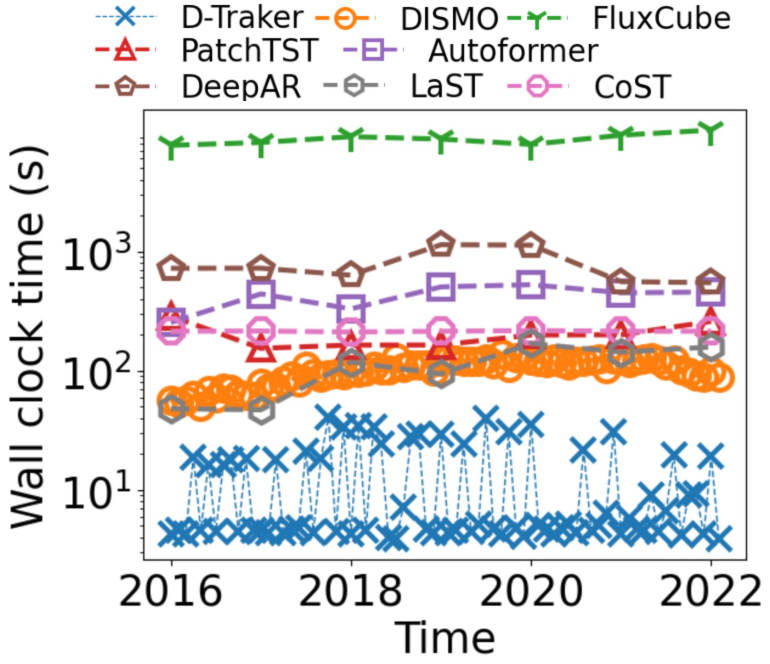
\includegraphics[width=\linewidth]{figures/scalability.png}
    \caption{Time versus stream length.}
  \end{subfigure}\hfill
  \begin{subfigure}[t]{0.49\linewidth}
    \centering
    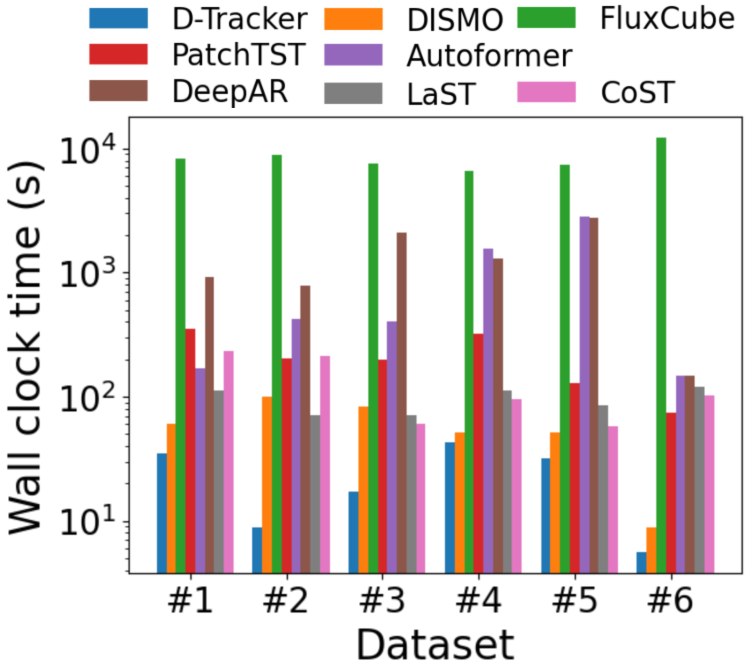
\includegraphics[width=\linewidth]{figures/avgtime.png}
    \caption{Average time over the streams.}
  \end{subfigure}
  \caption{D-Tracker scalability on Pythonlib. Source: Higashiguchi et al. (2025),
  arXiv:2505.00242v1, Figure~4; author-owned figure, CC BY 4.0.}
  \label{fig:scalability}
\end{figure}

In Figure~\ref{fig:scalability}, D-Tracker's processing time is nearly flat as the stream grows, while
baselines tend to rise. The small spikes occur when RankUpdate calls ModelEstimation several times.
This supports the ``time independent of stream length'' claim, but it is not a claim that every
operation is constant: cost still depends on keywords, locations, rank, and structure updates.

\subsection{Q3: is the model interpretable?}

\begin{figure}[htbp]
  \centering
  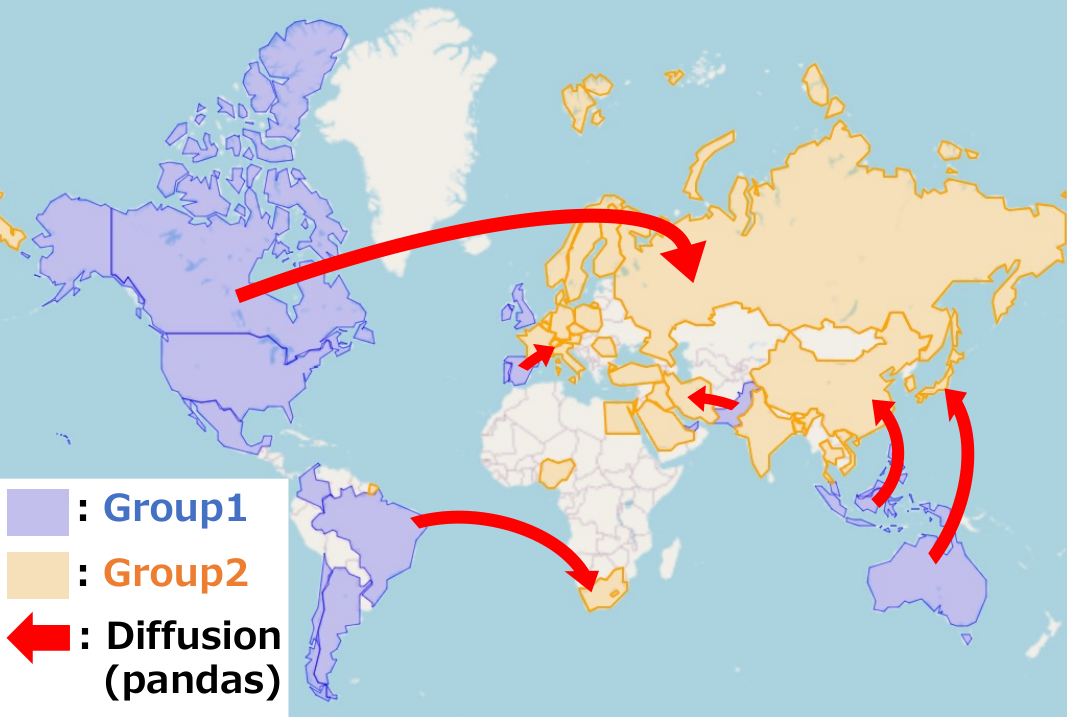
\includegraphics[width=0.78\linewidth]{figures/diff_2014.png}
  \caption{Part of the Pythonlib modeling result for 2013--2015: the reaction--diffusion system's
  diffusion pattern associated with ``pandas''. Source: Higashiguchi et al. (2025),
  arXiv:2505.00242v1, Figure~5; author-owned figure, CC BY 4.0.}
  \label{fig:diffusion-example}
\end{figure}

The paper reads Figure~\ref{fig:diffusion-example} as follows: the dynamics related to ``pandas''
spreads from a location group containing North America and Australia to a group containing Asian
countries, mainly China. This is a \emph{structured interpretation}: the keyword factor says
``pandas'', the location factor defines groups, and diffusion parameters give a direction. It is not
proof of causation; validation requires external evidence or an appropriate experimental design.

\subsection{What the paper does not establish}

The paper reports no confidence intervals, statistical significance tests, or predictive
probabilities. It also does not prove that D-Tracker always beats every baseline at every horizon; the
conclusion is bounded to six streams and the stated settings. The correct sentence is ``in these
experiments, D-Tracker achieved the best MAE and lower runtime'', not ``D-Tracker is the best method
for every time series''.

\begin{keypoint}
Remember three results: (1) D-Tracker leads MAE on all six datasets in paper Table~3; (2) per-step time does
not grow with stream length because of the fixed window, with spikes during rank changes; (3) the model
produces readable groups and diffusion directions, but these are interpretations under assumptions,
not proven causal effects.
\end{keypoint}

\begin{selfcheck}
\begin{enumerate}
  \item Why can MAE and RMSE rank two models differently?
  \item In the ablation, why might removing diffusion fail to hurt Language?
  \item Why does ``time independent of stream length'' not mean $O(1)$?
  \item State one conclusion that \emph{cannot} be drawn from Figure~\ref{fig:diffusion-example}.
\end{enumerate}
\end{selfcheck}

\section{Context and a critical reading}
\label{sec:discussion}

\subsection{Related work in one page}

The paper groups related work into three families. Understanding them shows what D-Tracker inherits
and what it tries to add.

\paragraph{Tensor analysis.}
Tucker, PARAFAC, and PARAFAC2 are standard tensor factorizations; online variants exist for large data.
MLDS combines a linear dynamical system with Tucker; SMF and SSMF focus on seasonality and forecasting.
DISMO combines PARAFAC with nonlinear differential equations and is interpretable, but it does
\emph{not} model diffusion across locations. D-Tracker adds that missing piece through
reaction--diffusion.

\paragraph{Time-series forecasting.}
Classical methods include autoregression and Kalman filters. Deep models use CNNs, RNNs, and
Transformers such as PatchTST and Autoformer; LaST/CoST learn trend/seasonal representations. They are
accurate on many tasks but hard to interpret and often expensive to retrain, which is awkward in a
stream.

\paragraph{Social-activity modeling.}
Earlier work models competition among search keywords. FluxCube uses physics-informed neural networks
to learn diffusion in temporal tensors, but repeatedly estimating location groups is expensive.
D-Tracker puts diffusion into a small ODE system and updates incrementally.

\begin{table}[htbp]
  \centering
  \scriptsize
  \caption{Capability comparison from paper Table~1. ``Yes'' means supported, ``--'' means not reported as
  supported. D-Tracker is the only method satisfying all six requirements in this table.}
  \label{tab:capabilities}
  \begin{tabular}{@{}lccccccc@{}}
    \toprule
    & DISMO & FluxCube & PatchTST & Autoformer & DeepAR & LaST/CoST & D-Tracker \\
    \midrule
    Forecasting & Yes & Yes & Yes & Yes & Yes & Yes & Yes \\
    Seasonality & Yes & Yes & -- & Yes & -- & Yes & Yes \\
    Diffusion & -- & Yes & -- & -- & -- & -- & Yes \\
    Independent of length & -- & -- & -- & -- & -- & -- & Yes \\
    Parameter free & Yes & -- & -- & -- & -- & -- & Yes \\
    Outlier & -- & -- & -- & -- & -- & -- & Yes \\
    \bottomrule
  \end{tabular}
\end{table}

\subsection{Genuine strengths}

The strength is not only ``more accurate forecasts''. D-Tracker combines three things that are usually
separate:
\begin{enumerate}
  \item a \textbf{generative} model with interpretable parameters (growth and diffusion between groups);
  \item a \textbf{streaming} mechanism that uses only the latest window;
  \item an \textbf{MDL} criterion that selects structure instead of manual trial and error.
\end{enumerate}
For an analyst, the benefit is the ability to ask, across a long series, ``which dynamics dominate,
for which groups, and in which direction?'' rather than receiving only a forecast.

\subsection{Assumptions and limitations to read alongside}

The following is this guide's assessment, not a set of results proven by the paper:

\begin{description}[leftmargin=1.8em,style=nextline]
  \item[Interpretation is not causation.] Reaction--diffusion is a \emph{structural assumption}. It can
  fit a delayed pattern caused by a third factor. The paper has no causal design, instrument, or
  intervention.
  \item[Additive three-part model.] Assuming
  $\mathcal{X}^{c}\approx\widehat{\mathcal{X}}_d+\widehat{\mathcal{X}}_s+\widehat{\mathcal{X}}_o$
  is strong. If trend and seasonality
  interact nonlinearly, or outliers are not sparse, the model may need too many outlier entries and
  lose interpretability.
  \item[Non-negative factors.] $\mathbf{W}\ge0$ makes groups readable and preserves signs, but limits
  relationships that require negative weights (for example, one keyword suppressing another) unless
  they are represented indirectly through several dynamics.
  \item[Non-identifiability.] Tensor factorizations are usually non-unique; groups may rotate or
  permute while reconstructing the same approximate tensor. Do not over-invest in the label ``Group
  1''; read relative structure and test stability.
  \item[Fixed window.] A fixed $L_c$ can miss cycles longer than the window or events from earlier
  history. Too-short or too-long windows both matter; the paper uses 104 weeks for GoogleTrends and 56
  days for Covid-19.
  \item[No uncertainty.] The model returns point forecasts, not confidence intervals or predictive
  distributions. High-stakes decisions need an uncertainty layer.
  \item[Missing/irregular data.] The paper does not present a formal mechanism for missing values,
  irregular timestamps, or changing location definitions. These are gaps to handle in application.
\end{description}

\subsection{How strong is the empirical evidence?}

The evidence has real strengths: six real streams, seven baselines, multiple horizons, component
ablations, and a runtime analysis. But read it with limits:
\begin{itemize}
  \item no statistical tests or confidence intervals for MAE differences;
  \item ``up to 57\%'' does not state its denominator at that point, so it is not a single effect size;
  \item the 8.0$\times$ speed-up depends on the paper's hardware and baseline training;
  \item ablations show that some components do not help on some datasets, as the paper acknowledges;
  \item the Covid-19 experiment has only two signals (cases and deaths) and does not represent all
        epidemiological dynamics.
\end{itemize}
None of this negates the results; it bounds the conclusions.

\subsection{When should D-Tracker be used?}

\textbf{Consider it} when data form a location/keyword-by-time tensor, short-horizon forecasting is
needed, group/diffusion hypotheses are useful, and updates should arrive with new data.

\textbf{Do not use it alone} for causal inference, under severe missing/irregular data, when calibrated
uncertainty is required, or when the tensor is so small that factorization offers no advantage. In
those settings D-Tracker can be a useful \emph{hypothesis generator}, not the final answer.

\subsection{Critical questions to prepare}

\begin{enumerate}
  \item If two regions rise together because of a global campaign, does the model always label it diffusion?
  \item As the number of regimes grows, how large can $\mathcal{F}$ become, and what is the memory cost?
  \item Are location groups stable across runs and initializations?
  \item What happens if $L_c$ is shorter than the seasonal period?
  \item Why use MDL rather than cross-validation for structure selection?
  \item Would the conclusions survive a different missing-value imputation?
\end{enumerate}
These are legitimate discussion questions, not proven flaws. The paper answers some partially; others
need additional experiments.

\begin{keypoint}
D-Tracker's value is in \textbf{connecting a generative model, MDL compression, and streaming}, not in
a single MAE number. A fair reading records the strong results while keeping their assumptions and
limits visible.
\end{keypoint}

\begin{selfcheck}
\begin{enumerate}
  \item Which capability in paper Table~1 is unique to D-Tracker?
  \item Why is ``diffusion did not help Language'' useful information rather than a flaw to hide?
  \item Name two assumptions that may fail when D-Tracker is applied to real data.
  \item If causal conclusions are required, what evidence must be added beyond this model?
\end{enumerate}
\end{selfcheck}


\appendix
\section{Learning aids and summary}
\label{app:learning}

\subsection*{D-Tracker on one page}

\begin{keypoint}
\textbf{Input:} a $k\times l\times L_c$ tensor window (keywords $\times$ locations $\times$ time).
\textbf{Output:} forecasts for $L_f$ steps and a readable model.
\textbf{Method:} split data into trend + seasonal + outlier; compress trend into a small core; evolve
the core with reaction--diffusion; estimate with ALS; select dimensions, outliers, and regimes with
MDL; update on a fixed window.
\end{keypoint}

\begin{enumerate}
  \item \textbf{Why is it hard?} Data are multi-dimensional with trend/seasonality/diffusion/outliers;
        patterns change over time; the stream is effectively unbounded.
  \item \textbf{Why split into three components?} To avoid confusing seasonality with trend and letting
        one shock corrupt every coefficient.
  \item \textbf{Why compress trend?} To turn tens of thousands of observations into a few latent
        dynamics and two keyword/location factor tables.
  \item \textbf{Why reaction--diffusion?} To represent both local growth and spread between location
        groups with meaningful parameters.
  \item \textbf{Why ALS?} Joint optimization is hard; alternating updates are easier to implement and
        preserve constraints.
  \item \textbf{Why MDL?} To select complexity with a principled criterion instead of manual search,
        and to decide outliers/regimes.
  \item \textbf{Why does streaming work?} Each step uses only the fixed $L_c$ window instead of
        rescanning the entire history.
  \item \textbf{What are the results?} The paper reports the best MAE on six datasets, nearly flat
        runtime as streams grow, and readable diffusion groups; it does not prove causation.
\end{enumerate}

\subsection*{A route back through the paper}

\begin{center}
\small
\begin{tabular}{@{}>{\raggedright\arraybackslash}p{0.27\linewidth}>{\raggedright\arraybackslash}p{0.31\linewidth}>{\raggedright\arraybackslash}p{0.34\linewidth}@{}}
  \toprule
  Read & Goal & Self-check \\
  \midrule
  Abstract + §1 & Grasp the problem, three properties, and Figure~1 & State the three challenges aloud \\
  §3.1 + paper Table~2 & Understand notation and Problem~1 & Write input/output in symbols \\
  §3.2--3.3 + Eq.~(1)--(4) & Understand decomposition and ODE & Explain every term in words \\
  §4.1 + Eq.~(5)--(9) & Understand ALS, LM, multiplicative updates & Recite the update order \\
  §4.2--4.3 + Eq.~(10) & Understand MDL and ModelUpdate & Explain the fit/complexity trade-off \\
  §5 + paper Table~3 + Figure~3--5 & Read results and ablations & Separate MAE/RMSE, claim, evidence \\
  Appendix A.1--A.4 & Initialization and algorithm details & Identify ambiguities \\
  \bottomrule
\end{tabular}
\end{center}

Suggested first-pass timing: 20 minutes for §1--3, 35 for §4, 25 for §5, and 20 for the appendix. You
need not follow every algebraic step immediately; first rewrite each equation as one English sentence.

\subsection*{Symbol table}

\begin{longtable}{@{}>{\raggedright\arraybackslash}p{0.23\linewidth}>{\raggedright\arraybackslash}p{0.35\linewidth}>{\raggedright\arraybackslash}p{0.35\linewidth}@{}}
  \caption{Symbols, shapes, and meaning.}\label{tab:appendix-symbols}\\
  \toprule
  Symbol & Shape & Meaning \\
  \midrule
  \endfirsthead
  \toprule
  Symbol & Shape & Meaning \\
  \midrule
  \endhead
  $k,l$ & integers & number of keywords, locations \\
  $t_c$ & time & current time \\
  $L_c,L_f$ & steps & window length, forecast horizon \\
  $\mathcal{X}^{c}$ & $k\times l\times L_c$ & current observed tensor \\
  $d_k,d_l$ & integers & number of keyword/location groups \\
  $d_s$ & integer & number of seasonal patterns \\
  $\mathcal{W}^{(\mathrm{core})}$ & $d_k\times d_l\times L_c$ & latent trend core \\
  $\mathbf{W}^{(\mathrm{key})}$ & $d_k\times k$ & non-negative keyword factors \\
  $\mathbf{W}^{(\mathrm{loc})}$ & $d_l\times l$ & non-negative location factors \\
  $\mathbf{A}$ & $d_k\times d_l$ & growth rates $a_{ij}$ \\
  $\mathcal{D}$ & $d_k\times d_l\times d_l$ & diffusion strengths $d_{ijj'}$ \\
  $\theta$ & --- & $\{\mathbf{A},\mathcal{D}\}$ \\
  $\theta_d,\theta_s$ & --- & trend parameters, seasonal parameters \\
  $\Theta$ & --- & one complete model \\
  $\mathcal{F}$ & --- & a set of regime models \\
  $\widehat{\mathcal{X}}_d,\widehat{\mathcal{X}}_s,\widehat{\mathcal{X}}_o$ & $k\times l\times L_c$ & trend, seasonal, outlier \\
  $\mathbf{S}^{(\mathrm{time})}$ & $d_s\times L_c$ & seasonal patterns over time \\
  $\mathbf{S}^{(\mathrm{key})},\mathbf{S}^{(\mathrm{loc})}$ & $d_s\times k$, $d_s\times l$ & seasonal factors \\
  \bottomrule
\end{longtable}

\subsection*{Vietnamese--English glossary}

\begin{longtable}{@{}>{\raggedright\arraybackslash}p{0.27\linewidth}>{\raggedright\arraybackslash}p{0.33\linewidth}>{\raggedright\arraybackslash}p{0.33\linewidth}@{}}
  \caption{Terms used in this guide.}\label{tab:glossary}\\
  \toprule
  Vietnamese & English & Brief note \\
  \midrule
  \endfirsthead
  \toprule
  Vietnamese & English & Brief note \\
  \midrule
  \endhead
  tensor & tensor & multi-dimensional array \\
  luồng tensor & tensor stream & sequence of tensors over time \\
  cửa sổ & window & most recent slice used for estimation \\
  tầm dự báo & forecast horizon & number of future steps \\
  phân rã tensor & tensor factorization & represent a tensor with smaller factors \\
  lõi & core & small tensor of latent dynamics \\
  nhân tố/hệ số & factor & strength of association with a group \\
  động học ẩn & latent dynamics & hidden series describing a pattern \\
  phản ứng & reaction & local growth/decay \\
  khuếch tán & diffusion & spread between groups \\
  mùa vụ & seasonality & repeating periodic pattern \\
  ngoại lai & outlier & unusual, sparse value \\
  chế độ & regime & period with relatively stable structure \\
  bình phương tối thiểu xen kẽ & alternating least squares (ALS) & optimize one block at a time \\
  mô tả ngắn nhất & minimum description length (MDL) & select by total bits \\
  không âm & non-negative & $\ge 0$ \\
  dự báo theo luồng & stream forecasting & forecast as data arrive \\
  độ phức tạp & computational complexity & how cost scales with size \\
  \bottomrule
\end{longtable}

\subsection*{Tiered self-check}

\paragraph{Tier 1 --- Recall and understanding.}
\begin{enumerate}
  \item What are D-Tracker's three components, and which pattern does each handle?
  \item Why must $\mathbf{W}^{(\mathrm{key})}$ and $\mathbf{W}^{(\mathrm{loc})}$ be non-negative?
  \item Which two costs make up MDL?
  \item Why does using only the latest window help in a stream?
\end{enumerate}

\paragraph{Tier 2 --- Apply and calculate.}
\begin{enumerate}
  \item With $d_k=3,d_l=2,L_c=104$, how many core entries are there? How many factor entries for
        $k=8,l=50$?
  \item If $w_{j'}=3,w_j=1,d_{jj'}=0.4,a_j=0$, what is the reaction--diffusion derivative?
  \item A model raises $d_s$ from 2 to 3: which way does model cost move, and why might fit improve?
\end{enumerate}

\paragraph{Tier 3 --- Critique.}
\begin{enumerate}
  \item Name a mechanism other than diffusion that could create a delayed pattern between countries.
  \item What may happen to the seasonal component if the window is shorter than the seasonal cycle?
  \item Why does ``best MAE'' not prove the model is best for every decision?
  \item What experiment would test whether location groups are stable?
\end{enumerate}

\subsection*{Suggested answers}

\paragraph{Tier 1.}
(1) Trend handles structured change and diffusion; seasonal handles repeating patterns; outlier handles
sparse unusual values. (2) So the projection cannot flip the sign of a dynamics and the reading
``this group rises/falls'' remains valid. (3) Model description cost plus data encoding cost.
(4) Per-step cost does not depend on total history, and the model can switch when patterns change.

\paragraph{Tier 2.}
(1) Core $3\cdot2\cdot104=624$; factors $3\cdot8+2\cdot50=124$. (2) $0+0.4(3-1)=0.8$.
(3) Model cost rises because there are more parameters; fit may improve because more seasonal patterns
can be represented, but the change survives only if total MDL falls.

\paragraph{Tier 3.}
(1) A global campaign, fast news, or a shared seasonal/event shock. (2) Seasonality may be absorbed
incorrectly into trend/outlier because the model does not see a full cycle. (3) MAE ignores uncertainty,
cost, interpretability, drift, and error distribution; risky decisions need intervals and tests.
(4) Run multiple initializations/seeds, compare groups across regimes, test coefficient stability, and
hold out entire locations.

\subsection*{Checklist before saying ``I understand the paper''}

\begin{itemize}
  \item I can redraw the pipeline from tensor to forecast without notes.
  \item I can explain Eq.~(1)--(4) in words, including tensor shapes.
  \item I can distinguish $\theta$, $\theta_d$, $\Theta$, and $\mathcal{F}$.
  \item I can state the roles of LM, multiplicative updates, ALS, and MDL.
  \item I can read paper Table~3 without confusing units and do not turn ``57\%'' into a firm conclusion.
  \item I can separate three things: paper results, model assumptions, and limits of the conclusions.
\end{itemize}

\section*{\DTReferencesName}
\addcontentsline{toc}{section}{\DTReferencesName}

\small
\begin{thebibliography}{99}

\bibitem{paper}
Shingo Higashiguchi, Yasuko Matsubara, Koki Kawabata, Taichi Murayama, and Yasushi Sakurai.
\newblock D-Tracker: Modeling Interest Diffusion in Social Activity Tensor Data Streams.
\newblock In \emph{KDD '25}, 2025.
\newblock DOI: \href{https://doi.org/10.1145/3690624.3709192}{10.1145/3690624.3709192};
arXiv: \href{https://arxiv.org/abs/2505.00242}{2505.00242}.
\newblock \emph{The primary source for every equation, figure, and reported value in this guide.}

\bibitem{kolda}
Tamara G. Kolda and Brett W. Bader.
\newblock Tensor decompositions and applications.
\newblock \emph{SIAM Review}, 51(3):455--500, 2009.

\bibitem{dismo}
Koki Kawabata, Yasuko Matsubara, and Yasushi Sakurai.
\newblock Modeling Dynamic Interactions over Tensor Streams.
\newblock In \emph{Proceedings of the ACM Web Conference 2023}, 1793--1803, 2023.

\bibitem{fluxcube}
Taichi Murayama, Yasuko Matsubara, and Yasushi Sakurai.
\newblock Mining Reaction and Diffusion Dynamics in Social Activities.
\newblock In \emph{CIKM '22}, 1521--1531, 2022.

\bibitem{patchtst}
Yuqi Nie, Nam H. Nguyen, Phanwadee Sinthong, and Jayant Kalagnanam.
\newblock A Time Series Is Worth 64 Words: Long-term Forecasting with Transformers.
\newblock arXiv:2211.14730, 2022.

\bibitem{autoformer}
Haixu Wu, Jiehui Xu, Jianmin Wang, and Mingsheng Long.
\newblock Autoformer: Decomposition Transformers with Auto-Correlation for Long-Term Series Forecasting.
\newblock In \emph{Advances in Neural Information Processing Systems 34}, 22419--22430, 2021.

\bibitem{deepar}
David Salinas, Valentin Flunkert, Jan Gasthaus, and Tim Januschowski.
\newblock DeepAR: Probabilistic Forecasting with Autoregressive Recurrent Networks.
\newblock \emph{International Journal of Forecasting}, 36(3):1181--1191, 2020.

\bibitem{last}
Zhiyuan Wang, Xovee Xu, Weifeng Zhang, Goce Trajcevski, Ting Zhong, and Fan Zhou.
\newblock Learning Latent Seasonal-Trend Representations for Time Series Forecasting.
\newblock In \emph{Advances in Neural Information Processing Systems 35}, 38775--38787, 2022.

\bibitem{cost}
Gerald Woo, Chenghao Liu, Doyen Sahoo, Akshat Kumar, and Steven Hoi.
\newblock CoST: Contrastive Learning of Disentangled Seasonal-Trend Representations for Time Series Forecasting.
\newblock arXiv:2202.01575, 2022.

\bibitem{stl}
Robert B. Cleveland, William S. Cleveland, Jean E. McRae, and Irma Terpenning.
\newblock STL: A Seasonal-Trend Decomposition Procedure Based on LOESS.
\newblock \emph{Journal of Official Statistics}, 6(1):3--73, 1990.
\newblock (The paper cites this as ``STL: A seasonal-trend decomposition''.)

\bibitem{ntd}
Yong-Deok Kim and Seungjin Choi.
\newblock Nonnegative Tucker Decomposition.
\newblock In \emph{IEEE Conference on Computer Vision and Pattern Recognition}, 1--8, 2007.

\bibitem{mdl}
Jorma Rissanen.
\newblock Modeling by Shortest Data Description.
\newblock \emph{Automatica}, 14(5):465--471, 1978.

\bibitem{lm}
Jorge J. Mor\'e.
\newblock The Levenberg--Marquardt Algorithm: Implementation and Theory.
\newblock In \emph{Numerical Analysis}, Springer, 105--116, 2006.

\end{thebibliography}

\begin{keypoint}
\ifdefstring{\DTExplainerLanguage}{vi}{%
  Tài liệu này không thay thế paper gốc. Khi có khác biệt giữa bản giải thích và nguồn, paper
  arXiv:2505.00242v1 là nguồn quyết định; các điểm mơ hồ đã được nêu trong các Chương~\ref{sec:model},
  \ref{sec:mdl-streaming} và~\ref{sec:experiments}.
}{%
  This document does not replace the original paper. If the guide and the source disagree, the
  source arXiv:2505.00242v1 decides; known ambiguities are surfaced in Sections~\ref{sec:model},
  \ref{sec:mdl-streaming}, and~\ref{sec:experiments}.
}
\end{keypoint}


\end{document}
